\documentclass[11pt,a4paper]{article}

\usepackage{../jedusor}

\usepackage[maxalphanames=99, maxnames=99, backend=bibtex, style=alphabetic, sorting=ynt]{biblatex}
\addbibresource{stage2A.bib}

\title{\textbf{Théorie K.A.M paradifférentielle}}
\date{}
\author{Sacha Ben-Arous, Mathis Bordet, \\ sous la direction de Thomas Alazard.\\ Stage de L3, ENS Paris-Saclay.}

% UTILISER GHYS DANS LINTRO
% \mathscr{F} pour joli Fourier


\begin{document}
\maketitle

\section{Introduction}
La théorie des systèmes dynamiques est née à la fin du 19ème siècle, sous l'impulsion des travaux d'Henri Poincaré sur le problème à 3 corps. Dans les années 50, Kolmogorov, suivi d'Arnold puis de Moser, bâtit une théorie de la dynamique des systèmes hamiltoniens et de leur perturbations, qui s'applique en particulier à la mécanique céleste. Le problème principal qui émerge de de ce type de dynamique est celui des ``\textit{petits diviseurs}'', qui se traduit par une perte de régularité induite par les opérateurs mis en jeu. La théorie K.A.M (Kolmogorov, Arnold, Moser) développe des outils raffinés d'analyse, en particulier le théorème de Nash-Moser, qui est un schéma de Newton modifié où sont rajoutés des opérateurs régularisants, afin de sumonter cette difficultée. \\
Ces résultats sont cependant difficiles d'accès de part leur sophistication (on présente en annexe une version succinte du théorème de Nash-Moser dûe à Hörmander \cite{hormander}), et d'autre part, les schémas itératifs utilisés ont pour conséquence de rendre physiquement irréalistes les ordres de grandeurs des perturbations prises en compte par la théorie. \\
Dans ce contexte, Thomas Alazard et Chengyang Shao publient une nouvelle preuve \cite{alazard} de certains résultats de K.A.M, qui utilise des outils de calcul paradifférentiel. Le principe de cette méthode est de directement régulariser les équations que l'on cherche à résoudre, puis de revenir à l'équation initiale à l'aide de théorèmes de point fixe. Cette approche a d'une part l'avantage d'être relativement élémentaire, et d'autre part les résultats de stabilité sont obtenus à partir de théorème de point fixe classiques et non plus avec des schémas itératifs, ce qui pourrait permettre d'améliorer la pertinence physique des bornes autorisées pour les perturbations. \\

Dans la première partie du rapport, nous présentons le cadre et les principaux théorèmes de la dynamique en dimension 1 sur le cercle, ainsi que des contre-exemples au théorème de Denjoy, afin d'observer l'optimalité de ce théorème. Pour cela, nous nous appuyons principalement sur \cite{dgv}, qui a par ailleurs aussi servi de support pour les parties suivantes. Dans la seconde partie, on pose les fondements du calcul paradifférentiel à l'aide de la décomposition de Littlewood-Paley, puis on énonce les théorèmes de paralinéarisation qui vont permettre de prouver un théorème dû à Arnold, qui permet de mettre en évidence le phénomène des petits diviseurs, et sa résolution à l'aide du calcul paradifférentiel.





\section{Difféomorphismes du cercle}
Nous allons dans cette section présenter rapidement les difféomorphismes du cercle et énoncer quelques propriétés fondamentales puisque ces objets nous offrent un cadre d'application des techniques de résolution d'équations que nous verrons dans les sections suivantes. On utilise les notations suivantes :
On note $\mathbb{S}^1$ le cercle de dimension 1 : $\left\{ z \in \mathbb{C} \mid |z|=1 \right\}$ et  $\Pi$ l'application $ t \to \exp (2i\pi t) $ (la projection de $\mathbb{R}$ sur $\mathbb{S}^1$).
\subsection{Problèmes de conjuguaison}
\begin{defin}
Soit $f :\mathbb{S}^1 \to \mathbb{S}^1$. On appelle relèvement de $f$, une application $F :  \mathbb{R} \to \mathbb{R}$ vérifiant :
\begin{equation*}
f \circ \Pi = \Pi \circ F.
\end{equation*}
\end{defin}
\begin{rmq}
Les relèvements permettent de faire le parallèle entre les fonctions du cercle et les fonctions réelles.
\end{rmq}
\begin{thm}
Toute application continue du cercle possède un relèvement continu. De plus, deux relèvements continus diffèrent d'une constante entière.
\end{thm}
Dans la suite, tous les relèvement d'applications continues du cercle seront pris continus.
\begin{defin}
Pour une application continue du cercle $f$, on définit son degré $deg(f) := F(1)-F(0)$ avec $F$ un relèvement de $f$.
\end{defin}
\begin{rmq}
Ce nombre est un entier relatif et il ne diffère pas selon les relèvements (continus).
\end{rmq}
\begin{defin}
On dit que $f$ préserve l'orientation si pour tout triangle avec ses sommets sur $\mathbb{S}^1$, l'image de ses sommets par $f$ n'inverse pas l'ordre de ses sommets.
\end{defin}
Ce qui nous intéressera dans la suite de cette étude sont surtout les homéomorphismes du cercle, qui sont les applications continues, bijectives et de réciproques continues (la dernière propriété est redondante du fait de la compacité de $\mathbb{S}^1$).

\begin{prop}
Prenons $f$ un homéomorphisme préservant l'orientation alors, $deg(f)=1$ et de plus ses relèvements sont croissants.
\end{prop}

\begin{prop}
Soit $f$ un homéomorphisme préservant l'orientation et $F$ un relèvement de $f$. Alors le nombre $\rho (F)=\displaystyle \lim\limits_{n \to +\infty} \frac{F^n(x)}{n}$ existe, ne dépend pas de $x$, et ne diffère que d'un entier relatif entre chaque relèvement.
\end{prop}

\begin{defin}
On définit alors le nombre de rotation de $f$ par $\rho(f) := \rho (F) \mod[1]$
\end{defin}
Cette quantité est fondamentale car elle caractérise le nombre de rotations moyen d'un homéomorphisme. On peut alors se demander si, de manière analogue à la relation de similitude en l'algèbre linéaire, il existe un représentant simple pour un homéomorphisme du cercle donné, i.e : un homéomorphisme du cercle $f$ est-il conjugué à la rotation d'angle $R_{\rho(f)}$ ? La réponse est clairement non si le nombre de rotation est rationnel : il suffit de remarquer qu'un homéomorphisme ayant un point fixe est de nombre de rotation nul, or la rotation d'angle $0$ est l'identité, et cette dernière est seule dans sa classe d'équivalence. Dans le cas irrationnel, le théorème suivant dû à Poincaré apporte une première réponse :
\begin{thm}[Poincaré]\label{poincare}
Soit $f$ un homéomorphisme préservant l'orientation, si son nombre de rotation est un irrationnel alors $f$ est semi-conjugué à la rotation d'angle $\rho(f)$, i.e : il existe une fonction du cercle $h$ continue, surjective, ayant un relèvement croissant, telle que $h\circ f = R_{\rho(f)} \circ h$.
\end{thm}
\begin{rmq}
La preuve de ce théorème utilise un résultat d'existence de mesure invariante pour une application continue du cercle, souvent appelé Théorème de Krylov-Bogolyubov. Or ce dernier n'est pas prouvé dans \cite{dgv}, et on propose donc une preuve inspirée d'un cours de Patrick Bernard en annexe.
\end{rmq}

Un critère d'inversibilité de la semi-conjuguaison est ensuite fourni par le théorème de Denjoy :
\begin{thm}[Denjoy]\label{denjoy}
En plus des hypothèses du théorème de Poincaré, si $f$ est $C^2$ alors $f$ est conjuguée à la rotation d'angle $\rho(f)$.
\end{thm}

On peut cependant se questionner sur la nécessité de l'hypothèse $C^2$ qui semble inattendue, et l'objet de la partie suivante sera de montrer que cette condition est optimale en un certain sens.


\subsection{Contres-exemples au théorème de Denjoy}
Cette partie est consacré à l'étude de certains contre-exemples du théorème de Denjoy, qui sont tirés du cours au Collège de France de Jean-Christophe Yoccoz de l'année 2013-2014, ainsi que du chapitre X de la thèse de Michel Herman \cite{herman} et du séminaire Bourbaki \cite{rosenberg} par Harold Rosenberg.

On se propose de montrer le théorème suivant :

\begin{thm}[Denjoy]\label{cex_denjoy}
Pour tout $\alpha \in \mathbb{R} \setminus \mathbb{Q}$, $\forall \epsilon > 0$, il existe un $\mathcal{C}^{2-\epsilon}$-difféomorphisme $f$ du cercle tel que $\rho(f)=\alpha$ et $f$ n'est pas conjugué à la rotation $R_\alpha$.
\end{thm}

\begin{rmq}
Ici, la  régularité non-entière est définie au sens de Hölder, i.e $f$ est $\mathcal{C}^1$, de dérivée $1-\epsilon$-hölderienne.
\end{rmq}

Pour construire un contre-exemple, on s'inspire de la preuve du théorème dans le cas $\mathcal{C}^2$ : on sait déjà par le \hyperref[poincare]{Théorème de Poincaré} qu'un tel $f$ est semi-conjugué à $R_\alpha$ par une fonction continue croissante $h$ du cercle. La preuve procède par l'absurde, en montrant que si $h$ n'est pas inversible, alors elle est constante sur un intervalle $I$ non trivial du cercle. Les itérés $f^n(I)$ sont alors disjoints (on dit que $I$ est un intervalle errant pour la dynamique de $f$), et on conclut en montrant que la somme de leurs tailles diverge. \\ 
L'idée ici est donc de construire une fonction $f$ qui admet un intervalle errant mais dont la suite des tailles des itérés de cet intervalle est sommable. 

\subsubsection{Outils}

On se servira de l'invariant de conjuguaison suivant : 

\begin{defin} 
Un homéomorphisme du cercle $f$ est dit \textit{minimal} si tout ensemble fermé invariant par  $f$ est vide ou égal au cercle tout entier. 
\end{defin}


\begin{prop}\label{minimal} ~
\begin{enumerate}
\item Si $f$ est conjugué à $g$ minimal, alors $f$ est minimal.
\item Si $\alpha \in \mathbb{R} \setminus \mathbb{Q}$, alors $R_\alpha$ est minimal
\end{enumerate}
\end{prop}

\begin{proof}
(1) est immédiat en utilisant la bicontinuité de la conjuguaison. \\
(2) s'obtient en remarquant que si $\alpha \in \mathbb{R} \setminus \mathbb{Q}$, alors $\alpha\mathbb{Z} + \mathbb{Z}$ est dense dans $\mathbb{R}$, et donc $\alpha\mathbb{Z}/\mathbb{Z}$ est dense dans le cercle $\mathbb{R}/\mathbb{Z}$. 
\end{proof}

La proposition suivante sera utile dans la suite :


\begin{prop}\label{dense}
Soient $D_1,D_2$ deux ensembles denses dans $[0,1]$, et $f : D_1 \to D_2$ une surjection croissante (resp. strictement croissante), alors $f$ admet un unique prolongement continu, croissant (resp. strictement croissant), de $[0,1]$ dans lui-même.
\end{prop}

\begin{proof}
L'unicité du prolongement est immédiate par densité de $D_1$, car deux fonctions continues sur un sous-ensemble dense sont partout égales. Si $x\in [0,1]\setminus D_1$, il existe $(x_n)_{n\in \mathbb{N}}$ dans $D_1$ qui tend vers $x$, que l'on peut supposer monotone. La suite $(f(x_n))_{n\in\mathbb{N}}$ est alors monotone bornée, donc converge vers une limite qui définit la valeur de $f(x)$.
% Cette définition ne dépend pas du choix de la suite, car si l'on se donne une autre suite $(\tilde{x}_n)_{n\in\mathbb{N}}$ ayant les mêmes propriétés, on remarque que la suite de terme général $f(x_n)-f(\tilde{x}_n)$ est de Cauchy. % 
Cette construction préserve clairement la monotonie (stricte) de $f$, et est de plus continue, car l'image monotone non continue d'un intervalle évite un intervalle, or l'image de $f$ est dense. 
\end{proof} 

\subsubsection{Contre-exemple continu} 

On note $(l_n)_{n\in \mathbb{Z}}$ la suite des longueurs des intervalles,  qui vérifie les propriétés suivantes : 
\begin{enumerate}

\item[(a)] $\displaystyle \sum_{n\in \mathbb{Z}} l_n = 1$ 

\item[(b)]$\displaystyle \lim\limits_{n \to \pm \infty } \frac{l_{n+1}}{l_n} = 1 $

\end{enumerate} On peut par exemple choisir $l_n = \displaystyle \frac{c}{n^2 + 1}$, où $c:=\displaystyle \frac{1}{\displaystyle \sum_{n\in\Z} \frac{1}{n^2+1}}$. \\
On note alors $ \alpha_n := \alpha n \mod 1$ et on pose $I_n := [b_n , c_n]$ où $\begin{cases} b_n := \displaystyle \sum_{\{m, \ \alpha_m < \alpha_n\}} l_m \\ c_n := \displaystyle \sum_{\{m, \ \alpha_m \leq \alpha_n\}} l_m  = b_n + l_n \end{cases}$ \\


\begin{lemma}\label{cantor}
L'ensemble $\displaystyle K := [0,1] \setminus \bigcup_{n\in \mathbb{Z}} \overset{\circ}I_n$ est un fermé non trivial.
\end{lemma}

\begin{proof}
Cet ensemble est clairement distinct de $[0,1]$, et il est de plus non vide car sinon, par compacité de $[0,1]$, on pourrait en extraire un recouvrement fini, mais alors la mesure de ce recouvrement serait strictement plus petite que $1$ au vu de la définition des $(I_n)_{n\in\mathbb{Z}}$, ce qui est absurde. 
\end{proof}


\begin{rmq}
$K$ est en fait un ensemble de Cantor, au sens où il est fermé d'intérieur vide et sans point isolé.
\end{rmq}

On considère ensuite la fonction $h$ définie par morceaux sur les $(I_n)_{n\in\mathbb{Z}}$, $h : I_n \mapsto \alpha_n$. 

\begin{lemma} 
Les $(I_n)_{n\in\mathbb{Z}}$ sont ordonnés identiquement aux $(\alpha_n)_{n\in\mathbb{Z}}$. De plus $h$ admet un prolongement continu sur $[0,1]$ qui vérifie $\forall n \in \mathbb{Z},\  h^{-1}(\{\alpha_n\})=I_n$
\end{lemma}


\begin{proof} \\
Soient $n_1,n_2 \in \mathbb{Z}$ tels que $\alpha_{n_1} < \alpha_{n_2}$, alors : $b_{n_2} - c_{n_1} = \displaystyle \sum_{k, \alpha_{n_1} < \alpha_k < \alpha_{n_2}} l_k \  > 0$, ce qui prouve le premier point. On en déduit immédiatement que $h$ est croissante, et alors par la \fcref{dense}, admet un prolongement continue croissant de [0,1] dans lui-même. \\
 Par définition, on a l'inclusion $I_n \subset h^{-1}(\{\alpha_n\})$. Si par l'absurde il existe $x$ tel que $h(x)=\alpha_n$ et $x \notin I_n$, alors $d(x,I_n) >0$. On suppose sans perte de généralité que $x<b_n$, alors par densité de $\displaystyle \bigcup_{n\in \mathbb{Z}} I_n$ il existe $y\in I_{n'}$ tel que $x\leq y < b_n$, et la croissance de $h$ donne $\alpha_n = h(x) \leq h(y) \leq \alpha_n$, i.e $\alpha_{n'} = \alpha_n$, ce qui est absurde, et donne donc l'égalité voulue. 
\end{proof}

On prolonge maintenant $h$ sur $\mathbb{R}$ par la relation, pour $x\in [0,1]$ et $p\in \mathbb{Z}$, $h(x+p)=h(x)+p$, et on note $I_{n,p}:=h^{-1}(\alpha_n+p)=I_n + p$. Alors $\displaystyle U:= \bigcup_{n,p \in \mathbb{Z}} \overset{\circ}I_{n,p}$ est un ouvert dense de $\mathbb{R}$, et $\mathbb{R}\setminus U$ est encore un ensemble de Cantor. \\

$\forall n \in \mathbb{Z}$, on choisit un homéomorphisme croissant $g_n$ de $I_n$ sur $I_{n+1}$, par exemple la transformation affine : $g_n(x) := \displaystyle \frac{l_n+1}{l_n}x + b_{n+1}-b_n\frac{l_{n+1}}{l_n}$, qui vérifie bien $g_n(b_n)=b_{n+1}$ et $g_n(c_n)=c_{n+1}$. Cela définit alors une application $g$ de $\displaystyle \bigcup_{n\in \mathbb{Z}} I_n$ dans lui-même, strictement croissante, que l'on prolonge sur $\mathbb{R}$ entier de la même manière que $h$. Par la \fcref{dense}, $g$ se prolonge en un homéomorphisme de $\mathbb{R}$ dans lui-même. On a alors par construction $h \circ g = R_\alpha \circ h$ sur $\displaystyle \bigcup_{n,p \in \mathbb{Z}} \overset{\circ}I_{n,p}$, mais cet ensemble est dense dans $\mathbb{R}$ et les fonctions en jeu sont continues, donc l'égalité a lieu sur tout $\mathbb{R}$. Par 1-périodicité de ces fonctions, elles descendent en applications du cercle, et on a la propriété suivante :

\begin{thm}\label{cont}
L'homéomorphisme du cercle $g$ construit précédemment vérifie $\rho(g)=\alpha$, mais $g$ n'est pas conjugué à $R_\alpha$.
\end{thm}

\begin{proof}
$\rho(g)=\alpha$ est immédiat car la semi-conjuguaison préserve le nombre de rotation (cf. \cite{dgv}).
Ensuite, $K = [0,1] \setminus \bigcup_{n \in \mathbb{Z}} \overset{\circ}I_{n}$ est invariant par $g$ par construction de ce dernier, mais cet ensemble est fermé non trivial d'après le  \fcref{cantor}, donc $g$ n'est pas minimal, et alors la \fcref{minimal} permet de conclure que $g$ n'est pas conjugué à $R_\alpha$. 
\end{proof}

\begin{centering}
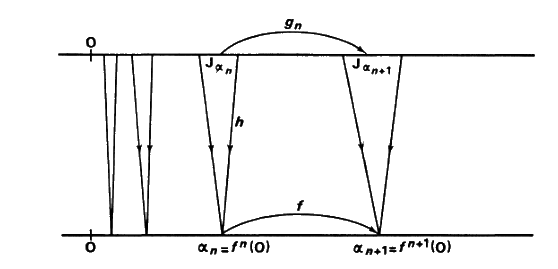
\includegraphics[scale=0.452]{diagram.png}
\captionof{figure}{\cite{herman} Schéma de la construction où $f=R_\alpha$}
\end{centering}

\subsubsection{Contre-exemple dérivable}

On considère toujours un homéomorphisme croissant $g_n$ de $I_n$ sur $I_{n+1}$, prolongé en $g_{n,p} = g_n +p$ sur $I_{n,p}$. On va de plus imposer que $g_n$ soit un difféomorphisme de classe $\mathcal{C}^1$, vérifiant : \\

$(*) \begin{cases}\ g_n'(x)=1 \ \text{ si } x \in \partial I_n \\ \displaystyle \lim_{n \to \pm \infty}\sup_{x\in I_n}|g_n'(x)-1|=0 \end{cases}$ \\

On considèrera enfin les fonctions $g_n'$ prolongées continuement sur tout l'intervalle [0,1], en les prenant constantes égales à 1 sur le complémentaire de $I_n$

\begin{lemma}
Les fonctions $\displaystyle g_n : x \mapsto b_{n+1} + \int_{b_n}^x 1 + \frac{6}{l_n^2}(\frac{l_{n+1}}{l_n} -1)(t-b_n)(c_n-t)\mathrm{d}t$ vérifient la condition $(*)$.
\end{lemma}

\begin{proof}
$g_n$ est un $\mathcal{C}^1$ difféomorphisme car sa dérivée est strictement positive. De plus, on a :
\begin{eqnarray*}
\int_{b_n}^{c_n} 1 + \frac{6}{l_n^2}(\frac{l_{n+1}}{l_n} -1)(t-b_n)(c_n-t)\mathrm{d}t &=& l_n +  \frac{6}{l_n^2}(\frac{l_{n+1}}{l_n} -1)\int_{b_n}^{c_n} (t-b_n)(c_n-t)\mathrm{d}t \\
&=& l_n +  \frac{6}{l_n^2}(\frac{l_{n+1}}{l_n} -1) \left [\frac{u^2}{2}l_n - \frac{u^3}{3}\right ]^{l_n}_0 \\
&=& l_n +  \frac{6}{l_n^2}(\frac{l_{n+1}}{l_n} -1) \frac{l_n^3}{6} = l_{n+1}
\end{eqnarray*}

Donc $g_n$ envoie bien $I_n$ sur $I_{n+1}$. La première condition de $(*)$ est immédiate, la seconde découle du fait que pour $x\in I_n$ : $ \displaystyle |g_n'(x) -1| \leq 6(\frac{l_{n+1}}{l_n} -1) \to 0 $ quand $n\to \pm \infty$ par hypothèse. 
\end{proof}

\begin{lemma}
La fonction $\eta$ qui coïncide avec $g_n'$ sur $I_n$ et qui vaut $1$ ailleurs est continue et vérifie $\displaystyle \eta =  1 + \sum_{n \in \mathbb{Z}} (g_n'-1)$
\end{lemma}

\begin{proof}
%On va montrer le résultat en utilisant la caractérisation séquentielle. Soit $x \in [0,1]$, et $(x_j)_{j\in \mathbb{N}}$ qui tend vers $x$.
%
%\underline{1er cas} : si il existe $n$ tel que $x \in \overset{\circ}I_{n}$, alors à partir d'un certain rang la suite  $(x_j)_{j\in \mathbb{N}}$ est dans $I_n$, et la continuité de $\eta$ se déduit de celle de $g_n'$. \\
%
%\underline{2ème cas} : si il existe $n$ tel que $x \in \partial I_{n}$, on va montrer que, sous réserve d'existence, la suite extraite $(x_{\varphi(j)})_{j\in \mathbb{N}}$ des termes dans $\displaystyle \bigcup_{n \in \mathbb{Z}} I_{n}$, et celle $(x_{\phi(j)})_{j\in \mathbb{N}}$ des termes qui n'y sont pas, ont une même limite par $\eta$ qui vaut $1=\eta(x)$. Par définition, on a $\forall j \in \mathbb{N}, \eta(x_{\phi(j)}) = 1$, ce qui donne une première limite.
En différenciant les cas $x \in I_n$, et $\displaystyle x\in [0,1] \setminus \bigcup_{n \in \mathbb{Z}} I_n$, l'égalité ponctuelle est immédiate. On va de plus montrer que la convergence est uniforme, ce qui donnera la continuité de $\eta$. \\ 
Soit $N \in \mathbb{N}$, et $x\in [0,1]$, on a : $\displaystyle \sum_{|k| \geq N} (g_n'(x)-1)= \begin{cases} g_n'(x)-1 \ \text{ si il existe } n \text{ tel que } x\in I_n \text{ et } |n|\geq N\\ 0 \end{cases}$ \\
Dans tous les cas, $\displaystyle \sup_{x\in [0,1]} \left | \sum_{|k| \geq N} (g_n'(x)-1) \right | \leq \sup_{|n| \geq N} |g_n'(x) -1|$. Or par hypothèse sur les dérivées, ce majorant tend vers $0$ et donc la convergence est uniforme. 
\end{proof}

La fonction $g$ admet comme dans la partie précédente un prolongement en homéomorphisme de [0,1] mais on a cette fois le résultat plus fort suivant :

\begin{thm}
$g$ est un difféomorphisme de classe $\mathcal{C}^1$ qui vérifie $\rho(g)=\alpha$ mais n'est pas conjugué à $R_\alpha$.
\end{thm}


\begin{proof}
Le seul point qui ne découle pas du \fcref{cont} est que $g$ est un $\mathcal{C}^1$-difféomorphisme. Pour montrer cela, on commence par remarquer que $g$ est d'une part continue, et que d'autre part $g$ est un $\mathcal{C}^1$-difféomorphisme sur $\displaystyle U := \bigcup_{n,p\in \mathbb{Z}} I_{n,p}$ qui est de mesure pleine dans $\mathbb{R}$. \\
Alors, si $A$ est un borélien de mesure de Lebesgue nulle, on a $\lambda(g(A)) \leq \lambda(g(A\cap (\mathbb{R} \setminus U))) + \lambda(g(A\cap U))$. 
Or le premier terme est nul car $\mathbb{R} \setminus U$ est stable par $g$ et de mesure nulle, et le second terme est nul par théorème de changement de variable, $g$ étant un $\mathcal{C}^1$-difféomorphisme sur $ U $, et $A$ de mesure nulle. \\

On en déduit que la mesure de Stieltjes associée à $g$ est absolument continue par rapport à la mesure de Lebesgue. Ainsi $g$ admet une dérivée de Radon-Nikodym $\mu \in \mathcal{L}^1(\mathbb{R})$, telle que $g(x) = g(0) + \displaystyle \int_0^x \mu(t) \mathrm{d}t$. Mais alors $\mu$ est presque partout égale à $g_n'$ sur les $(I_{n,p})_{p\in \mathbb{Z}}$ d'après la théorie des points de Lebesgue, i.e presque partout égale à $\eta$ car $U$ est de mesure pleine, et on a finalement : $g(x) = g(0) + \displaystyle \int_0^x \eta(t) \mathrm{d}t$. \\
On en déduit que $g$ est un homéomorphisme $\mathcal{C}^1$ de $\mathbb{R}$ à dérivée non nulle, et donc un $\mathcal{C}^1$-difféomorphisme. 
\end{proof}

\subsubsection{Régularité hölderienne}

Soit $w:[0, 1] \mapsto [0, 1]$ un module de continuité, on considère l'ensemble des fonctions continue pour ce module, $\displaystyle\mathcal{C}^w(\mathbb{T}) := \left\{ \varphi \in \mathcal{C}^0(\mathbb{T}) \ \left| \ \sup_{ 0<|x-y|\leq 1}  \frac{|\varphi(x)-\varphi(y)|}{w(|x-y|)} < +\infty \right. \right\} $ \\

En considérant la fonction $g$ construite dans la partie précédente, on a le lemme :

\begin{lemma}\label{reg_holder}
$ \displaystyle \sup_{n\in \mathbb{Z}} \left |\frac{l_{n+1}}{l_n}-1 \right |\frac{1}{w(l_n)} <+ \infty \Rightarrow g' \in \mathcal{C}^w(\mathbb{T})$
\end{lemma}

\begin{proof}
 On suppose sans perte de généralité que $w(x)/x$ est décroissante. En reprenant le $g_n'$ de la construction précédente, on constate que :  \\

$\displaystyle |g_n''(t)| = \frac{6}{l_n^2}(\frac{l_{n+1}}{l_n}-1)|(c_n-t + b_n -t)| \leq  \frac{3}{l_n}(\frac{l_{n+1}}{l_n}-1) $ \\

L'inégalité des accroissements finis donne donc : \\

$\displaystyle \sup_{0<x-y\leq 1} \left | \frac{g_n'(x) - g_n'(y)}{w(x-y)}\right | \leq \left | \frac{l_{n+1}}{l_n}-1\right | \frac{3}{w(l_n)} < +\infty$, et on en déduit que $g' \in \mathcal{C}^w(\mathbb{T})$ car $g'-1$ est limite uniforme de $\displaystyle  \sum_{k = -n}^n (g_k'-1)$, et les fonctions dans la somme ayant des supports disjoints 2 à 2, on a :\\

$\displaystyle  \left | \sum_{k = -n}^n (g_k'-1) \right |_{\mathcal{C}^w} \leq 2\sup_{n \in \mathbb{Z}} |g_n' -1|_{\mathcal{C}^w} \leq \frac{6}{l_n}(\frac{l_{n+1}}{l_n}-1) < + \infty $ 
\end{proof}

La suite $ \displaystyle l_n := \frac{c}{(|n|+k)(log(|n| + k)^{1+\epsilon}}$ vérifie le critère du \fcref{reg_holder} pour le module $w(x)=O(x^{1-\epsilon'})$, pour tout $\epsilon' > \epsilon$, ce qui permet de conclure la preuve du \fcref{cex_denjoy}

\section{Calcul paradifférentiel}
Cette partie a pour objectif d'exposer les principaux théorèmes de paralinéarisation de Bony \cite{bony}, avec pour point de départ la décomposition de Littlewood-Paley, et comme but de démontrer un théorème dû à Arnold, que l'on énonce dans un second temps. On s'appuiera sur \cite{metivier}, \cite{dgv}, et \cite{alinhac_gerard} comme références, en particulier les chapitres 4 et 5 du livre de Métivier.

\subsection{Décomposition de Littlewood-Paley}
Nous allons dans cette section présenter la décomposition de Littlewood-Paley. C'est une décomposition de fonction dans laquelle chaque terme a un spectre borné. Nous allons également présenter des propriétés sur cette décomposition. 
\begin{defin}[Transformée de Fourier]
On note $\mathcal{F} : L^1(\R^d) \to C^0_0(\R^d)$,  $\ \mathcal{F}f(\xi) := \displaystyle \int_{\R^d} e^{-2i\pi \xi \cdot x}f(\xi)\mathrm{d}x$, et on pourra utiliser la notation $\hat{f}$ pour désigner $\mathcal{F}f$. On manipulera de plus le prolongement usuel de $\mathcal{F}$ à l'espace des distributions tempérées $\mathcal{S}'(\R^d)$.
\end{defin}
On s'intéresse dans un premier temps à l'existence et, plus précisément, à la construction de fonctions $C^\infty(\mathbb{R}^d)$ avec un support au voisinage de 0 mais également constantes au voisinage de 0.

Considérons le cas $d=1$ et notons  $g: \R^+ \to \R$
\[ g(x) = \begin{cases} 
1 & \text{si } 0 \leq x \leq \frac{1}{2} \\
\exp\left(-\frac{1}{\frac{1}{4} - |x - \frac{1}{2}|^2}\right) & \text{si } \frac{1}{2} \leq x \leq 1 \\
0 & \text{sinon} \end{cases}
\]
On a alors que $g$ appartient à $C^\infty(\mathbb{R})$ puisqu'on peut montrer par récurrence que :
\begin{equation}\label{plateau}
\forall n \in \mathbb{N}^*, \ \forall x \in \left[\frac{1}{2}, 1\right], \ g^{(n)}(x) = x Q_n(|x|) \exp\left(-\frac{1}{\frac{1}{4} - |x - \frac{1}{2}|^2}\right)
\end{equation}
avec $Q_n$ une fraction rationnelle dont le pôle se situe en 1 , ce qui montre la continuité des $(g^{(n)})_{n \in \mathbb{N}}$ par croissances comparées. On étend alors cette construction à $\mathbb{R}^d$ en notant $\psi(x)=g(|x|)$, qui est une fonction $C^\infty(\R^d)$ avec $\text{supp}(\psi) \subset B(0,1)$ et est égale à 1 sur $B(0,\frac{1}{2})$. \\
En posant $\chi(x)=\psi(x)-\psi\left(\frac{x}{2}\right)$, on a ainsi $\text{supp}(\chi(2^{-k} \cdot)) \subset B(0,2^{k+1}) \setminus B(0,2^{k-1})$, et par téléscopage on obtient l'égalité  :
\begin{equation*}
 \forall \xi \in \mathbb{R}^d, \ 1= \psi(\xi) + \sum_{k=0}^\infty \chi(2^{-k} \xi)
\end{equation*}

\begin{lemma}\label{decomp}
Pour tout $u \in \mathcal{S}$ on a :
\[ \hat{u} = \psi \hat{u} + \sum_{k=0}^\infty \chi(2^{-k} \cdot) \hat{u} \]
et la série converge dans l'espace de Schwartz.
\end{lemma}
\begin{proof}
Soit $u \in \mathcal{S}$, montrons que pout tout $\alpha$ et $\beta \in \mathbb{N}\times \mathbb{N}^d $, $\left\lVert x^\alpha \partial^\beta(u-\psi(2^{-k}x)u) \right\rVert_\infty \to_{k\to \infty} 0$
On considère pour cela :
\begin{align*}
    \left\lVert x^\alpha \partial^\beta(u-\psi(2^{-k}x)u)\right\rVert_\infty &= \left\lVert x^\alpha \partial^\beta(u-\psi(2^{-k}x)u)\right\rVert_{\infty,[2^{k-1};2^{k+1}]} \\
    &\leq \left\lVert x^\alpha \partial^\beta u\right\rVert_{\infty,[2^{k};2^{k+1}]} + \left\lVert x^\alpha \partial^\beta u(1-\psi(2^{-k}x)\right\rVert_{\infty,[2^{k-1};2^{k}]}
\end{align*}

Comme $u \in \mathcal{S}$, on a $\left\lVert x^\alpha \partial^\beta u\right\rVert_{\infty,[2^{k};2^{k+1}]}$ qui tend bien vers $0$ lorsque $p$ tend vers $+\infty$. En utilisant la formule de derivation de Leibniz sachant que $\partial^j \psi = O(x^{j})$ (en utilisant \eqref{plateau}) on a que $\left\lVert x^\alpha \partial^\beta u(1-\psi(2^{-k}x)\right\rVert_{\infty,[2^{k-1};2^{k}]}$ tend bien vers $0$ lorsque $p$ tend vers $+\infty$. Pour conclure on utilise finalement que la transformée de Fourier est une bijection de $\mathcal{S}$ dans lui-même.
\end{proof}

\begin{defin}
On définit les opérateurs de la décomposition de Littlewood-Paley de la manière suivante :
\[
\text{Pour } u \in \mathcal{S}', \quad \widehat{\Delta_{-1} u} := \psi \cdot \hat{u}, \quad \widehat{\Delta_{k} u} := \chi(2^{-k} \cdot) \cdot \hat{u} \ \text{ si } k \geq 0
\]
\end{defin}

\begin{prop}
Soit $u \in \mathcal{S}'$, en posant :
\[ S_n u := \sum_{k=-1}^{n-1} \Delta_k u \]
On a que :
\[ \lim_{n \to \infty} S_n u = u \]
où la convergence est au sens de $\mathcal{S}'$.
\end{prop}
\begin{rmq}
Dans la suite, pour simplifier les calculs, il nous arrivera d'écrire $S_{-k}$ pour $k\geq 0$, et dans ce cas on prend comme définition $S_{-k} := S_{0} = \Delta_{-1}$.
\end{rmq}

\begin{proof}
Prenons $u \in \mathcal{S}'$ et $v \in \mathcal{S}$.
\[ \langle \mathcal{F}(S_n u), v \rangle = \langle \psi(2^{-n}\xi) \mathcal{F}(u), v \rangle = \langle \mathcal{F}(u), \psi(2^{-n}\xi) v \rangle \]
Or, $\lim_{n \to +\infty} \psi(2^{-n}\xi)v = v$ dans $\mathcal{S}(\mathbb{R}^d)$ par le \fcref{decomp}. On obtient donc :
\[ \mathcal{F}(S_n u) \to \mathcal{F}(u) \quad \text{dans} \ \mathcal{S}' \]
Par continuité de $\mathcal{F}^{-1}$, on a finalement $S_n u \to u$ quand $n \to +\infty$.
\end{proof}
     
     
\begin{defin}[Espaces de Sobolev]
Pour tout $s\in \R^+$, on définit 
\begin{equation*}
H^s(\R^d) := \left\{ u\in L^2(\R^d), \xi \mapsto (1+|\xi|^2)^{\frac{s}{2}}\hat{u}(\xi) \in L^2(\R^d) \right\}
\end{equation*}
et on admet que c'est un espace de Hilbert muni de la norme $\|u\|_{H^s} := \displaystyle \left(\int_{\R^d} (1+|\xi|^2)^s\hat{u}(\xi)^2\mathrm{d}\xi \right)^\frac{1}{2}$
\end{defin}


\begin{defin}[Espaces de Zygmund]
Pour tout $\alpha > 0$, on définit 
\begin{equation*}
C^\alpha_*(\R^d) := \left\{ u\in L^\infty(\R^d), \sup_{k \geq -1} 2^{k\alpha}\|\Delta_ku\|_{L^\infty} < +\infty \right\}
\end{equation*}
et on admet que c'est un espace de Banach muni de la norme $\|u\|_{C^\alpha_*} :=  \sup_{k \geq -1} 2^{k\alpha}\|\Delta_ku\|_{L^\infty} $
\end{defin}

\begin{lemma}[Inégalité de Bernstein]
Soit $B$ une boule, $1\leq p  \leq  q \leq +\infty$, $k\in \N$, et $\lambda >0$. Si $u\in L^p$ est tel que $\text{supp}(\hat{u})\subset \lambda B$, alors
\begin{equation}\label{bernstein}
\max_{|\alpha|=k}{\| \partial^\alpha u\|_{L^q}} \ \lesssim_k \lambda^{|\alpha| +d \left ( \frac{1}{p}- \frac{1}{q} \right )}\|u\|_{L^p}
\end{equation}
\end{lemma}

\begin{proof}
On commence par justifier que $u\in \mathcal{S}$. En effet, $u$ ayant un spectre borné, sa transformée de Fourier est dans l'espace de Schwartz, et l'opérateur transformée de Fourier étant un automorphisme de $\mathcal{S}$ dans lui-même, on en déduit que $u\in \mathcal{S}$. \\
Soit $\varphi \in C^\infty_c(\R^d)$ qui vaut 1 sur un voisinage de $B$, on a $\hat{u}(\xi)=\varphi(\lambda^{-1}\xi)\hat{u}(\xi)$, donc $u=\lambda^d u * g$, avec $g := \mathcal{F}^{-1}(\varphi)(\lambda \cdot)$, et donc $\partial^\alpha u =\lambda^d u * \partial^\alpha g$. L'inégalité de Young donne de plus que : $\|f * g \|_{L^q} \leq \|f\|_{L^p} \|g\|_{L^r}$, où $1\leq p,r\leq q \leq +\infty$, et $\frac{1}{p}+\frac{1}{r}= 1 + \frac{1}{q}$. Or :
\begin{eqnarray*}
\| \partial^\alpha g \|^r_{L^r} &=& \int_{\R^d} \left | \partial^\alpha \left(\mathcal{F}^{-1} \varphi(\lambda x)\right) \right |^r \mathrm{d}x =   \lambda^{|\alpha|r} \int_{\R^d} \left | \partial^\alpha \left(\mathcal{F}^{-1}(\varphi)\right)(\lambda x) \right |^r \mathrm{d}x  \\
&\leq& \lambda^{|\alpha|r-d} \| \partial^\alpha \mathcal{F}^{-1}\varphi \|^r_{L^r}
\end{eqnarray*}
Ce qui donne bien :
\begin{eqnarray*}
\| \partial^\alpha u \|_{L^q} \leq \lambda^{|\alpha| + d(1-\frac{1}{r})} \| \partial^\alpha \mathcal{F}^{-1}\varphi \|_{L^r} \|u\|_{L^p} = C_k\lambda^{|\alpha| + d(\frac{1}{p}-\frac{1}{q})} \|u\|_{L^p}
\end{eqnarray*}
\end{proof}


\begin{lemma}\label{young}
Il existe $C>0$ tel que pour tout $1\leq p \leq +\infty$, $u \in L^p(\R^d)$, 
\begin{align*}
\sup_{n\geq -1}\|S_nu\|_{L^p} &\leq C \|u\|_{L^p} & \sup_{k\geq -1}\|\Delta_ku\|_{L^p} &\leq C \|u\|_{L^p}
\end{align*}
\end{lemma}

\begin{proof}
On écrit $S_n u = 2^{nd} (\mathcal{F}^{-1}\psi)(2^n\cdot)\star u$. Par inégalité de Young on obtient :
$$\left\lVert S_n u \right\rVert_{L^p} \leq \left\lVert u \right\rVert_{L^p} \left\lVert 2^{nd} (\mathcal{F}^{-1}\psi)(2^n\cdot) \right\rVert_{L^1}$$ 
Or, par changement de variable, on obtient : 
\begin{align*}
 \left\lVert 2^{nd} (\mathcal{F}^{-1}\psi)(2^n\cdot) \right\rVert_{L^1} &= 2^{nd} \int_{\R^d} \left| (\mathcal{F}^{-1}\psi)(2^nx)  \right| \mathrm{d}x \\
 &= \int_{\R^d} \left| \mathcal{F}^{-1}\psi(x) \right| \mathrm{d}x = \|\mathcal{F}^{-1}\psi\|
\end{align*}
On procède de même pour $\|\Delta_k u\|_{L^p}$.
\end{proof}

\begin{lemma}[Presque-orthogonalité]\label{lqortho}
Pour tout $u\in L^2(\R^d)$, 
\begin{equation}\label{qortho}
\sum_{k \geq -1} \|\Delta_k u \|^2_{L^2} \leq \| u \|^2_{L^2} \leq 2 \sum_{k \geq -1} \|\Delta_k u \|^2_{L^2} 
\end{equation}
\end{lemma}

\begin{proof}
On part de $1= \psi(\xi) + \sum_{p=0}^\infty \chi(2^{-p} \xi)$.
Seule deux de ces fonctions ont une intersection de support non vide. On utilise alors : $a^2 +b^2 \leq (a+b)^2 \leq 2(a^2 +b^2)$ et on obtient:
$$ \frac{1}{2} \leq \psi(\xi)^2 + \sum_{p=0}^\infty \chi(2^{-p} \xi)^2 \leq 1$$
La seconde inégalité de \eqref{qortho} s'en déduit en multipliant l'inégalité ci-dessus par $\hat{u}$ et en utilisant l'identité de Plancherel.
\end{proof}

\begin{prop}[Caractérisation des espaces de Sobolev]\label{prop_carac_sobolev}
Si $s\in \R^+$, $u\in L^2(\R^d)$, on a alors $u\in H^s(\R^d) \Leftrightarrow \sum_{k\geq -1}2^{2ks}\|\Delta_k u \|_{L^2}^2 < +\infty$. De plus, il existe $C>0$ tel que :
\begin{equation}\label{carac_sobol}
\frac{1}{C}\sum_{k\geq -1}2^{2ks}\|\Delta_k u \|_{L^2}^2 \leq \|u\|_{H^s}^2 \leq C \sum_{k\geq -1}2^{2ks}\|\Delta_k u \|_{L^2}^2 
\end{equation}
\end{prop}

\begin{proof}
En notant $\left\langle \xi \right\rangle = \sqrt{1 + |\xi|^2}$, on a $\|u\|_{H^s} = \|\left\langle D \right\rangle^su\|_{L^2}$, et le \fcref{lqortho} donne 
\[\sum_{k \geq -1} \|\Delta_k \left\langle D \right\rangle^su \|^2_{L^2} \leq \| u \|^2_{H^s} \leq 2 \sum_{k \geq -1} \|\Delta_k \left\langle D \right\rangle^su \|^2_{L^2} \]
La formule de Plancherel et la définition de $\Delta_k$, on obtient l'existence de $C>0$ tel que $\forall k \geq -1$
\[\frac{1}{C}2^{ps}\|\Delta_ku\|_{L^2} \leq  \|\Delta_k\left\langle D \right\rangle^su\|_{L^2} \leq C2^{ps}\|\Delta_ku\|_{L^2} \]
et donc il existe $\tilde{C}$ tel que :
\[
\frac{1}{\tilde{C}}\sum_{k\geq -1}2^{2ks}\|\Delta_k u \|_{L^2}^2 \leq \|u\|_{H^s}^2 \leq \tilde{C} \sum_{k\geq -1}2^{2ks}\|\Delta_k u \|_{L^2}^2 \]
ce qui donne l'équivalence des normes voulue.
\end{proof}

\begin{lemma}[Injection de Sobolev]\label{inject}
Soit $s>\frac{d}{2}$, si $u\in H^s(\R^d)$ alors $u\in C^{s-\frac{d}{2}}_*(\R^d)$, en particulier $u\in L^\infty(\R^d)$, et pour tout $k\in \N$ :
\begin{equation*}
\|\Delta_ku\|_{L^\infty} \lesssim 2^{k(\frac{d}{2}-s)} \|u\|_{H^s}
\end{equation*}
\end{lemma}


\begin{proof}
Soit $u\in H^s(\R^d)$, d'après le résultat précédent on sait que pour tout $k\in \N$, $\Delta_ku\in L^2(\R^d)$, donc sa transformée de Fourier y est de même, et comme elle est à support compact, elle est dans $L^1(\R^d)$. D'après la formule d'inversion, on a ainsi : 
\begin{equation*}
\Delta_ku(x) = \frac{1}{(2\pi)^d}\int_{\R^d} e^{i x\cdot \xi} \widehat{\Delta_ku}(\xi)\mathrm{d}\xi
\end{equation*}
Alors, l'inégalité de Cauchy-Schwarz donne :
\begin{align*}
\|\Delta_ku\|_{L^\infty} \leq \|\Delta_ku\|_{L^2} \left|B(0,C 2^k) \right| ^\frac{1}{2} &\lesssim 2^{k(\frac{d}{2}-s)} 2^{ks}\|\Delta_ku\|_{L^2} \leq 2^{k(\frac{d}{2}-s)} (\sum_{k\geq -1} 2^{ks}\|\Delta_ku\|^2_{L^2})^{\frac{1}{2}} \leq 2^{k(\frac{d}{2}-s)} \|u\|_{H^s}
\end{align*}
Ce qui consitue l'inégalité voulue. On en déduit immédiatement que $\sup_{k \geq -1} 2^{k({s-\frac{d}{2}})}\|u\|_{L^\infty} \leq \|u\|_{H^s}$, et donc $u\in C^{{s-\frac{d}{2}}}_*$. De plus, on en déduit que la série de terme général $(\Delta_ku)_{k\in \N}$ est absolument convergente dans $L^\infty$, donc par complétude elle converge simplement vers un $\tilde{u}$. On a déjà vu que cette série converge dans $\mathcal{S}'$ vers $u$, donc $u=\tilde{u} \in L^\infty(\R^d)$.
\end{proof}


\begin{prop}\label{spec_ball}
Soit $(u_k)_{k\geq -1}$ tel que $\exists R >0, \forall k\geq -1, \text{supp }\hat{u}_k \subset B(0,R2^k)$. \\
\begin{itemize}
\item[•]Soit $\alpha >0$, si $\sup 2^{k\alpha}\|u_k\|_{L^\infty} < +\infty$, alors $u=\sum u_k \in C^\alpha_*(\R^d)$, et 
\begin{equation*}
\|u\|_{C^\alpha_*} \leq C\sup_k 2^{k\alpha}\|u_k\|_{L^\infty}
\end{equation*}
\item[•]Soit $s >0$, si $\sum 2^{2ks}\|u_k\|^2_{L^2} < +\infty$, alors $u=\sum u_k \in H^s(\R^d)$, et 
\begin{equation*}
\|u\|_{H^s}^2 \leq C\sum_k 2^{2ks}\|u_k\|^2_{L^2} 
\end{equation*}
\end{itemize}
\end{prop}

\begin{proof}
Par hypothèse sur le support des $(u_k)_{k\geq -1}$, pour tout $q \geq -1$,  en notant $N := \lfloor\log_2(R) \rfloor + 1$, on a: 
\begin{equation*}
\Delta_q u = \sum_{k\geq q-N} \Delta_qu_k
\end{equation*}
On en déduit :
\begin{equation*}
2^{q\alpha}\|\Delta_qu\|_{L^\infty}\leq  2^{q\alpha}\sum_{k\geq q-N}\|\Delta_qu_k\|_{L^\infty} \leq 2^{q\alpha}\sum_{k\geq q-N}\|u_k\|_{L^\infty} \leq \sum_{k\geq q-N} 2^{k\alpha}\|u_k\|_{L^\infty} 2^{(q-k)\alpha} \leq \sum_{k\in \Z} a_k b_{q-k}
\end{equation*}
où :
\begin{itemize}
\item[•] $a_k =  2^{k\alpha}\|u_k\|_{L^\infty}$ si $k\geq -1$, $a_k = 0$ sinon.
\item[•] $b_r =  2^{r\alpha}$ si $r\leq N$, $b_r = 0$ sinon.
\end{itemize}
Comme $\alpha>0$, $(b_r)_{r\in \Z}$ est sommable, et l'inégalité de Young discrète donne :
\begin{equation*}
\|2^{k\alpha}\|\Delta_ku\|_{L^\infty}\|_{\ell^\infty} \leq \|a_q\|_{\ell^\infty} \|b_r\|_{\ell^1}
\end{equation*}
i.e :
\begin{equation*}
\|u\|_{C^\alpha_*} = \sup_k 2^{k\alpha}\|\Delta_ku\|_{L^\infty} \leq C\sup_k 2^{k\alpha}\|u_k\|_{L^\infty} 
\end{equation*}
On conclut alors par définition des espaces de Zygmund. La preuve dans le second cas est parfaitement analogue, en remplaçant $\alpha$ par $s$, et l'espace $L^\infty$ par $L^2$.
\end{proof}


\begin{prop}[]\label{meyer}
Soit $s>0$, $n\in \N$, $n>s$. Il existe $C$ tel que pour toute famille $(u_k)_{k\in \N}$ dans $H^n(\R^d)$, si pour tout $\alpha \in \N^d$, avec $\ |\alpha| \leq n $ :
\begin{equation*}
\|\partial ^\alpha u_k \|_{L^2} \leq 2^{k(|\alpha|-s)}\varepsilon_k
\end{equation*}
où $(\varepsilon_k)_{k\in \N} \in \ell^2(\N)$, alors la somme $u:=\sum_k u_k \in H^s(\R^d) $, et $ \|u\|_{H^s}^2 \leq C \sum_k \varepsilon_k^2 $.
\end{prop}

\begin{proof}
On remarque que la série de terme général $u_k$ est absolument convergente dans $L^2$, donc par complétude elle converge simplement, et $u$ est bien définie. Ensuite : 
\begin{equation*}
2^{js}\|\Delta_ju\|_{L^2} \leq \sum_{k\geq j} 2^{js}\|\Delta_ju_k\|_{L^2} + \sum_{k < j} 2^{js}\|\Delta_ju_k\|_{L^2}
\end{equation*}
Par hypothèse, et en utilisant le \fcref{young}, on a d'une part :
\begin{equation*}
\|\Delta_ju_k\|_{L^2} \leq C \|u_k\|_{L^2} \leq C2^{-ks}\varepsilon_k
\end{equation*}
D'autre part, en utilisant l'inégalité de Bernstein \eqref{bernstein}, on obtient pour tout $j\geq 0$ :
\begin{equation*}
\|\Delta_ju_k\|_{L^2} \leq C 2^{-nj} \sum_{|\alpha|=n} \|\partial^\alpha\Delta_ju_k\|_{L^2} \leq C 2^{-nj} \|u_k\|_{H^n} \leq C 2^{-(j-k)n}2^{-ks}\varepsilon_k
\end{equation*}
Alors :
\begin{equation*}
2^{js}\|\Delta_ju\|_{L^2} \leq C \sum_{k\geq j} 2^{(j-k)s}\varepsilon_k + C \sum_{k < j} 2^{(j-k)(s-n)}\varepsilon_k = C (a \star \varepsilon)_j
\end{equation*}
où le dernier membre est une convolution discrète entre $\varepsilon = (\varepsilon_k)_{k\in \Z}$ et  $a = (a)_{k\in \Z}$ avec
\[a_k=2^{ks} \text{ si } k \leq 0, \quad a_k=2^{k(s-n)} \text{ sinon.}\]
Comme $a\in \ell^1(\Z)$, l'inégalité de Young discrète donne que $(2^{js}\|\Delta_ju\|_{L^2})_{j\in \N}$ est de carré sommable, ce qui donne le résultat voulu d'après la caractérisation de la \fcref{prop_carac_sobolev}. \\
\end{proof}


\begin{cor}[Multiplicateurs de Meyer]\label{true_meyer}
Soient $r,s>0$, $n\in\N$ tel que $n>s$. Si $(m_k)_{k \geq -1}$ est une suite de $L^\infty(\R^d)$ telle que pour tout multi-indice $\alpha$ avec $|\alpha|\leq n$, on ait :
\begin{equation*}
\|\partial^\alpha m_k\|_{L^\infty} \leq M_\alpha 2^{k(|\alpha|-r)},
\end{equation*}
alors l'opérateur 
\begin{equation*}
f \mapsto \sum_{k\geq -1} m_k\Delta_kf
\end{equation*}
est continu de $H^s(\R^d)$ dans $H^{s+r}(\R^d)$, et sa norme est bornée par $C_s\displaystyle \sum_{|\beta|\leq n} M_\beta$.
\end{cor}

\begin{proof}
Pour tout $|\alpha|\leq n$, on a 
\begin{align*}
\|\partial^\alpha (m_k\Delta_kf)\|_{L^2} &\leq C_\alpha \sum_{\beta \leq \alpha} \|\partial^\beta m_k\|_{L^\infty} \|\partial^{\alpha-\beta}\Delta_kf\|_{L^2} \\
&\leq C_\alpha 2^{k(|\alpha|-r-s)}\left(\sum_{\beta\leq \alpha} M_\beta \right)2^{ks}\|\Delta_kf\|_{L^2}.
\end{align*}
Alors, la \fcref{meyer} permet d'aboutir au résultat voulu.
\end{proof}
\subsection{Estimations douces et paralinéarisation}
On va maintenant se servir de la décomposition de Littlewood-Paley pour étudier des produit dans les espaces fonctionnels précédemment utilisés. On remarque que l'on peut écrire, pour $u,v \in \mathcal{S}(\R^d)$ : 
\begin{align*}
uv &=\sum_{k,j}\Delta_ku\Delta_jv = \sum_{k=-1}^{+\infty}\sum_{j=-1}^{p}\Delta_ku\Delta_jv + \sum_{k=-1}^{+\infty}\sum_{j=k+1}^{+\infty}\Delta_ku\Delta_jv \\
&=\sum_{k=-1}^{+\infty}\Delta_kuS_{k+1}v +  \sum_{j=0}^{+\infty}\sum_{k=-1}^{j-1}\Delta_ku\Delta_jv = \sum_{k=-1}^{+\infty}\Delta_kuS_{k+1}v +  \sum_{j=-1}^{+\infty}\Delta_jvS_{j}u \\
&= \sum_{k=-1}^{+\infty}\Delta_kuS_{k-2}v  \ +  \sum_{k=-1}^{+\infty}\Delta_kvS_{k-2}u \ + \sum_{|k-j|\leq 2} \Delta_ku\Delta_ju \\
&= T_vu + T_uv + R(u,v)
\end{align*}
Ici, $T_vu$ (resp. $T_uv$) décrit la partie des interactions pour lesquelles la fréquence de $v$ (resp. $u$) est nettement plus faible que celle de $u$ (resp. $v$), tandis que $R(u,v)$ représente la partie où les fréquences sont du même ordre. Le terme $T_vu$ est appelé \textit{paraproduit} de $u$ par $v$.
\begin{prop}[Estimations douces pour les paraproduits et leurs restes]\label{tame} ~\\
\begin{itemize}
\item[•] $\forall s\in \R^+, u \in L^\infty, v\in H^s,$
\begin{equation}\label{estim1}
\|T_uv\|_{H^s} \leq C_s \|u\|_{L^\infty} \|v\|_{H^s}
\end{equation}
\item[•] $\forall \alpha \in \R^+, u \in L^\infty, v\in C^\alpha_*,$
\begin{equation}\label{estim2}
\|T_uv\|_{C^\alpha_*} \leq C_\alpha \|u\|_{L^\infty} \|v\|_{C^\alpha}
\end{equation}
\item[•] $\forall r,s\in \R^+$ tels que $r+s>0, u \in C^r_*, v\in H^s,$
\begin{equation}\label{estim3}
\|R(u,v)\|_{H^{r+s}} \leq C_{r,s} \|u\|_{C^r_*} \|v\|_{H^s}
\end{equation}
\item[•] $\forall \alpha,\beta\in \R^+$ tels que $\alpha + \beta>0, u \in C^\alpha_*, v\in C^\beta_*,$
\begin{equation}\label{estim4}
\|R(u,v)\|_{C^{\alpha + \beta}_*} \leq C_{\alpha,\beta} \|u\|_{C^\alpha_*} \|v\|_{C^\beta_*}
\end{equation}
\end{itemize}
\end{prop}

\begin{proof}
On remarque que $T_uv$ a une décomposition qui vérifie les hypothèses de la \fcref{spec_ball}. En effet, $T_uv=\sum_{p=-1}^{+\infty}S_{p-2}u\Delta_pv$, et le spectre de $S_{p-2}u\Delta_pv$ est inclus dans $B(0,2^{p-2})+B(0,2^{p+1}) \subset B(0,4\times2^p)$. Alors, le \fcref{young} et la \fcref{prop_carac_sobolev} donnent :
\begin{align*}
\sum_k 2^{2ks} \|\Delta_kvS_{k-2}u \|^2_{L^2} &\leq \sum_k 2^{2ks} \|\Delta_kv \|^2_{L^2} \|S_{k-2}u\|_{L^\infty} \leq C \|u\|_{L^\infty}^2 \sum_k 2^{2ks} \|\Delta_kv \|^2_{L^2} \\
&\leq  C' \|u\|_{L^\infty}^2 \|v\|_{H^s}^2
\end{align*}
On conclut alors que $\|T_uv\|_{H^s} \leq C_s \|u\|_{L^\infty} \|v\|_{H^s}$ à l'aide de la \fcref{spec_ball}. Les inégalités suivantes se montrent de manière parfaitement analogue.
\end{proof}
%
%\begin{prop}[Estimations douces pour le produit] ~\\
%\begin{itemize}
%\item[•] $\forall s>0,\ u,v \in L^\infty \cap H^s(\R^d)$,
%\begin{equation*}
%\|uv\|_{H^s} \leq C (\|u\|_{L^\infty}\|v\|_{H^s} + \|v\|_{L^\infty}\|u\|_{H^s})
%\end{equation*}
%\item[•] $\forall \alpha \in \R^+ \setminus \N,\ u,v \in C^\alpha_*(\R^d)$,
%\begin{equation*}
%\|uv\|_{C^\alpha_*} \leq C (\|u\|_{L^\infty}\|v\|_{C^\alpha_*} + \|v\|_{L^\infty}\|u\|_{C^\alpha_*})
%\end{equation*}
%\end{itemize}
%\end{prop}


\begin{thm}[Paralinéarisation]\label{paralin}
Soit $F$ une fonction $C^{\infty}$ de $\R$ telle que $F(0)=0$. Si $u\in H^s(\R^d)$, avec $\rho := s - \frac{d}{2}>0 $, alors 
\begin{equation}
F(u) - T_{F'(u)}u \in H^{s+\rho}(\R^d).
\end{equation}
\end{thm}
Pour prouver ce théorème, on commence par montrer le lemme suivant : 


\begin{lemma}\label{lem_paralin}
Soit $F$ une fonction $C^{\infty}$ de $\R$ telle que $F(0)=0$. Si $u\in H^s(\R^d)\cap L^{\infty}(\R^d) $, avec $s\geq 0 $, alors $F(u) \in H^s(\R^d)$ et 
\begin{equation}
\|F(u)\|_{H^s} \leq C_s \|u\|_{L^{\infty}} \|u\|_{H^s}
\end{equation}
\end{lemma}


\begin{proof}
Si $s=0$, le résultat se déduit de l'existence d'une fonction $G$ continue telle que $F(u)=uG(u)$. Alors, comme $u\in L^2$ et $G(u) \in L^{\infty}$ car $u$ est bornée, on obtient bien $F\in L^2$. \\
Quand $s>0$, on remarque qu'il existe $C_\alpha$  indépendant de $u$ et $k$ telle que  : 
\begin{equation}\label{ineq_l2}
\|\partial^\alpha \Delta_k u \|_{L^2} \leq C_\alpha 2^{(|\alpha|-s)k} \varepsilon_k
\end{equation}
avec $\sum \varepsilon_k^2 =  \|u\|_{H^s}^2$. En effet, l'inégalité de Bernstein (\ref{bernstein}) puis la caractérisation des espaces de Sobolev (\ref{carac_sobol}) donnent le résultat voulu. On a de plus,
\begin{equation}\label{ineq_unif}
\|\partial^\alpha \Delta_k u \|_{L^{\infty}} \leq C_\alpha 2^{|\alpha|k} \|u\|_{L^{\infty}}
\end{equation}
toujours par l'inégalité de Bernstein. Le lemme de presque-orthogonalité (\ref{qortho}) donnant que $(\Delta_k u)_{k\in \N}$ est terme général d'une série absolument convergente, la complétude de $L^2$ fournit alors la convergence simple de cette série, i.e. $S_nu \to u$ dans $L^2$. De plus, d'après le \fcref{young},  $\|S_pu\|_{L^\infty} \leq C \|u\|_{L^\infty}$. On en déduit que $F(S_nu) \to F(u)$ dans $L^2$ car :
\[ \| F(S_nu) - F(u)\|_{L^2} \leq C \sup_{t\in[0,1]} \|F'(tS_nu- (1-t)u \|_{L^\infty}\|S_nu-u\|_{L^2} \to 0 \]
Un argument télescopique donne alors : 
\begin{equation}\label{telesc}
F(u) = F(S_0 u) + \sum_{k=0}^{+\infty} F(S_{k+1} u) - F(S_k u) = F(S_0 u) + \sum_{k=0}^{+\infty} m_k \Delta_k u
\end{equation}
où \[m_k := \int_0^1 F'(S_ku + t\Delta_ku)\mathrm{d}t\]
Alors, on obtient dans un premier temps que : 
\begin{equation*}
\| \partial^\alpha F'(S_ku + t\Delta_ku)\|_{L^{\infty}} \leq C_{\alpha,F} 2^{|\alpha|k} \|u\|_{L^{\infty}}
\end{equation*}
Pour cela on utilise la règle de la chaine (plus précisement la formule de Faà di Bruno), on majore uniformément les termes en $F'$ avec le \fcref{young} et on utilise (\ref{ineq_unif}) pour les termes en $u$.
En intégrant, on obtient alors :
\begin{equation}\label{majint}
\|\partial^\alpha m_k \|_{L^\infty} \leq C_{\alpha,F} 2^{|\alpha|k} \|u\|_{L^{\infty}}
\end{equation}
Donc par la formule de Leibniz et l'inégalité (\ref{ineq_l2}), on obtient :
\begin{equation*}
\|\partial^\alpha(m_k \Delta_k u) \|_{L^2} \leq C_{\alpha,F} 2^{(|\alpha|-s)k} \|u\|_{L^{\infty}} \varepsilon_k
\end{equation*}
On peut donc conclure par la \fcref{meyer}.
\end{proof}


\begin{proof}[Preuve du \fcref{paralin}]On commence par remarquer que quitte à soustraire un terme linéaire $au$ à $F(u)$, on peut supposer que $F'(0)=0$. Cela ne change rien à la preuve car :
\[F(u)+au - T_{F'(u) + a}u = F(u) + au - T_{F'(u)}u  -T_{a}u =  F(u) + au - T_{F'(u)}u  -au =  F(u) - T_{F'(u)}u \]
Ensuite, comme $\rho >0$, le \fcref{inject} donne $u\in L^\infty(\R^d)$. Par définition, on a \[T_{F'(u)}u = S_{-3}F'(u)\cdot u_0 + \sum_{k=0}^\infty S_{k-2} F'(u)\cdot \Delta_k u \]
En utilisant (\ref{telesc}), comme $F(S_0u)$ et $S_{-3}F'(u) \cdot u_0$ sont dans $H^\infty$, il suffit de prouver que :
\[\sum_{k=0}^\infty(m_k-S_{k-2}g)\Delta_k u \ \in H^{s+\rho}\]
Cela découle de la \fcref{meyer}, que l'on peut appliquer d'une part grâce à (\ref{ineq_l2}), et d'autre part car on a l'inégalité :
\begin{equation*}
\| \partial^\alpha (m_k - S_{k-2}F'(u))\|_{L^\infty} \leq C_\alpha 2^{(|\alpha|-\rho)k}
\end{equation*} 
Pour obtenir cette dernière, on va montrer séparément :
\begin{align}
\| \partial^\alpha (m_k - F'(S_{k-2}u))\|_{L^\infty} &\leq C_\alpha 2^{(|\alpha|-\rho)k} \label{eq1} \\
\| \partial^\alpha (F'(S_{k}u) - S_kF'(u))\|_{L^\infty} &\leq C_\alpha 2^{(|\alpha|-\rho)k} \label{eq2}
\end{align}
On commence par écrire la formule de Taylor avec reste intégral, qui donne 
\[F'(S_ku+t\Delta_ku)-F'(S_{k-2}u)=\mu_kw_k\]
avec 
\begin{equation*}
w_k=(\Delta_{k-2}u + \Delta_{k-1}u + t\Delta_ku) \quad \text{ et } \mu_k = \int_0^1F''(S_{k-2}u + \tau w_k)\mathrm{d}\tau.
\end{equation*}
De manière analogue à \eqref{majint}, on a 
\begin{equation*}
\|\partial^\alpha \mu_k \|_{L^\infty} \leq C_{\alpha,F} 2^{|\alpha|k} \|u\|_{L^\infty}
\end{equation*}
Tandis que $w_k$ vérifie
\begin{equation*}
\| \partial^\alpha w_k\|_{L^\infty} \leq C_{\alpha} 2^{\frac{d}{2}k} \| \partial^\alpha w_k\|_{L^2} \leq C_{\alpha} 2^{\frac{d}{2}k} 2^{(|\alpha|-s)k} \varepsilon_k  \leq \tilde{C}_{\alpha} 2^{(|\alpha|-\rho)k}
\end{equation*}
où l'on a utilisé l'inégalité de Bernstein \eqref{bernstein}, puis \eqref{ineq_l2}. On en déduit donc que 
\begin{equation*}
\|\partial^\alpha (\mu_kw_k)\|_{L^\infty} \leq C_\alpha 2^{(|\alpha|-\rho)k} 
\end{equation*}
Or 
\begin{equation*}
m_k - F'(S_{k-2}u) = \int_0^1 \mu_k w_k\mathrm{d}t
\end{equation*}
Ce qui donne \eqref{eq1}.
Pour montrer la seconde inégalité, on commence par décomposer en deux membres le terme à majorer :
\begin{equation*}
\left[ F'(S_{k}u) - S_k F'(S_{k}u) \right] + \left[ S_k F'(S_{k}u) - S_kF'(u) \right] = (\rom{1}) + (\rom{2})
\end{equation*}
L'inégalité de Bernstein \eqref{bernstein} donne alors 
\begin{equation*}
\|\partial^\alpha S_k (F'(u) - F'(S_ku) )\|_{L^\infty} \lesssim_\alpha 2^{(|\alpha| + \frac{d}{2})k } \|S_k (F'(u) - F'(S_ku) )\|_{L^2}.
\end{equation*}
De plus :
\begin{equation*}
\|S_k (F'(u) - F'(S_ku) )\|_{L^2} \lesssim \|F'(u) - F'(S_ku) )\|_{L^2} \lesssim \|u-S_ku\|_{L^2} \lesssim 2^{-ks}\|u\|_{H^s}
\end{equation*}
grâce au \fcref{young}, puis aux accroissements finis, et finalement avec une majoration du reste géométrique dans la caractérisation des espaces de Sobolev \eqref{carac_sobol}. Ainsi $(\rom{2})$ vérifie l'inégalité \eqref{eq2}. \\
Il reste maintenant à étudier $(\rom{1})$. Pour cela, on remarque que $S_ku \in H^\infty$ car sa transformée de Fourier est à support compact. Alors, d'une part $S_ku \in L^\infty	$ par le \fcref{young} car $u\in L^\infty$, et sa norme est bornée indépendamment de $k$. D'autre part, en écrivant la norme usuelle de Sobolev et en utilisant l'inégalité de Bernstein, on a que pour tout $N \in \N$ :
\begin{align*}
 \|S_ku\|_{H^{s+N}} &\leq C\|S_ku\|_{H^s} + C\sum_{|\alpha|=s+N} \|\partial^\alpha S_k u \|_{L^2} \\
& \leq \|S_ku\|_{H^s} + C_{\alpha,N} 2^{kN} \|S_ku\|_{H^s} \\
& \leq C_{\alpha,N} 2^{kN}\|u\|_{H^s} .
\end{align*}
où l'on a observé que $\|S_ku\|_{H^s} \leq \|u\|_{H^s}$ à partir de l'écriture utilisant les multiplicateurs de Fourier, et avec la norme de Sobolev adaptée. Alors, le \fcref{lem_paralin} donne que $F'(S_ku)\in H^{s+N}$, et 
\begin{equation}\label{utillem}
\|F'(S_ku)\|_{H^{s+N}} \leq C_{\alpha,N}2^{kN}\|u\|_{H^s}\|u\|_{L^\infty}
\end{equation}
En utilisant l'inégalité de Bernstein puis le \fcref{inject}, on remarque que pour $\sigma > |\alpha| + \frac{d}{2}$ et $a\in H^\sigma(\R^d)$,
\begin{equation*}
\|\partial^\alpha \Delta_j a\|_{L^\infty} \leq C 2^{j(\frac{d}{2}-\sigma+|\alpha|)} \|a\|_{H^\sigma}
\end{equation*}
Et alors, comme $a-S_ka=\sum_{j\geq k} \Delta_j a$, par majoration d'un reste géométrique, on a :
\begin{equation}\label{aled}
\|\partial^\alpha (a-S_k a)\|_{L^\infty} \leq C 2^{k(\frac{d}{2}-\sigma+|\alpha|)} \|a\|_{H^\sigma}
\end{equation}

En appliquant \eqref{aled} avec $a=F'(S_ku)$ et $\sigma = s + N$ où $N$ est suffisamment grand pour que $s+N > \frac{d}{2} + |\alpha|$, on a 
\begin{align*}
\|\partial^\alpha (F'(S_ku)-S_k F'(S_ku))\|_{L^\infty} &\leq C 2^{k(\frac{d}{2}-s-N+|\alpha|)} \|F'(S_ku)\|_{H^{s+N}} \\
& \leq  C_{\alpha,N} 2^{k(\frac{d}{2}-s+|\alpha|)} \|u\|_{H^s}
\end{align*}
où l'on a utilisé \eqref{utillem}, ce qui donne finalement la majoration attendue pour $(\rom{1})$, conclut la preuve de l'inégalité \eqref{eq2} et achève donc la preuve du \fcref{paralin}.
\end{proof}

\begin{thm}[Paralinéarisation des produits]\label{paralin_prod}
Soit $s,r>0$, et $a,b\in C^r_*(\T^d)$. Alors 
\begin{equation*}
R_{CM}(a,b) := T_a \circ T_b - T_{ab}
\end{equation*}
est un opérateur continu de $H^s(\T^d)$ dans $H^{s+r}(\T^d)$, et on a :
\begin{equation*}
\|R_{CM}(a,b)\|_{\mathcal{L}(H^s,H^{s+r})} \leq C_{s,r} \|a\|_{C^r_*}\|b\|_{C^r_*}
\end{equation*}
\end{thm}

\begin{proof}
Soit $u\in H^s(\R^d)$, on note $v:=T_bu$ et $v_k:=S_{k-2}b\cdot\Delta_ku$. On observe que :

\begin{align*}
T_aT_bu - \sum_j \sum_{k \leq j-3} \Delta_ka\cdot v_j &= \sum_j S_{j-2}a\cdot\Delta_jv - \sum_j \sum_{k \leq j-3} \Delta_ka\cdot v_j \\
&=\sum_j \sum_{k \leq j-3} \Delta_ka\cdot (\Delta_jv - v_j) \\
&=\sum_k \Delta_ka \sum_{k+3 \leq j \leq k+5} (\Delta_jv - v_j) 
\end{align*}
Car $\sum_qv_q=\sum_q\Delta_qv$, et que $v_q$ a un spectre inclus dans la boule de rayon $2^q$. En développant la défintion de $v_j$, et en utilisant le \fcref{true_meyer}, on a :
\begin{equation}\label{aled1}
\left\| T_aT_bu - \sum_j \sum_{k_1 \leq j-3} \sum_{k_2\leq j-3} \Delta_{k_1}a\cdot \Delta_{k_2}b \cdot \Delta_j u \right\|_{H^{s+r}} \leq C_{s,r} \|a\|_{C^r_*} \|b\|_{C^r_*} \|u\|_{H^s}
\end{equation}
De plus, en notant 
\begin{equation*}
c_j := \sum_{k_1 \leq j-3}\sum_{k_2 \leq j-3}\Delta_{k_1}a \cdot \Delta_{k_2}b,
\end{equation*}
on a :
\begin{align*}
\|ab-c_j\|_{L^\infty} &\leq \sum_{k_1\geq j-3 \text{ ou } k_2 \geq j-3}\|\Delta_{k_1}a\|_{L^\infty} \cdot \|\Delta_{k_2}b\|_{L^\infty} \\
&\leq C_r \|a\|_{C^r_*} \|b\|_{C^r_*} \sum_{k_1+k_2 \geq j-3} 2^{-(k_1+k_2)r} \\
&\leq C_r \|a\|_{C^r_*} \|b\|_{C^r_*}  2^{-jr} 
\end{align*}
Or :
\begin{equation*}
T_{ab}u-\sum_jc_j \cdot \Delta_ju = \sum_j(S_{j-2}(ab) - c_q) \cdot \Delta_ju,
\end{equation*}
et en utilisant les deux inégalités précédentes avec le \fcref{true_meyer}, il vient :
\begin{equation}\label{aled2}
\left\| T_{ab}u-\sum_jc_j\cdot \Delta_ju \right\|_{H^{s+r}} \leq C_{s,r} \|a\|_{C^r_*} \|b\|_{C^r_*} \|u\|_{H^s}
\end{equation}
En combinant \eqref{aled1} et \eqref{aled2}, on conclut la démonstration du théorème.
\end{proof}

\subsection{Théorème d'Arnold}
On s'intéresse dans cette section au cas suivant : $g$ difféomorphisme du cercle régulier (au moins $C^2$), préservant les angles et ayant un angle de rotation $\alpha$ irrationnel. On a automatiquement par le \fcref{denjoy} qu'il est conjugué à la rotation d'angle $\alpha$. Le théorème d'Arnold s'intéresse à la régularité de la conjugaison lorsque $g$ est "très proche" de la rotation $R_\alpha$.
\subsubsection{Description du problème}
On choisit de réecrire $g$ comme une perturbation de la rotation soit: $g= f + R_\alpha$ avec $f$ "assez petit" (nous définirons ce que cela veut dire dans la suite). On cherche alors naturellement la conjugaison que l'on note $\eta$, l'équation à résoudre est alors :

\begin{equation}\label{arnold1}
\eta(x + \alpha)= \eta(x) + \alpha + f \cdot \eta(x) \\
\end{equation}
On écrit la conjuguaison sous la forme d'une perturbation de l'identité soit $\eta=id+u$. \\
Pour plus de généralité on introduit ici un paramètre réel $\lambda$ et en utilisant les notations de $\eta$ avec $u$, l'équation \eqref{arnold1} devient:
\begin{equation}\label{arnold2}
\Delta_\alpha u= f \cdot (id +u) - \lambda \; \text{avec  } \Delta_\alpha u(x)= u(x+\alpha) - u(x)
\end{equation}
d'inconnue $u$.
\par Pour illustrer le problème de régularité que va poser ce type d'équation, intéressons-nous d'abord à l'équation \eqref{arnold2} linéarisée:
\begin{equation}\label{arnold3}
\mu + \Delta_\alpha v = h 
\end{equation}
avec $\mu= \text{Avg } h$. \\
En utilisant les séries de Fourier, on obtient la solution suivante:
\begin{equation*}
\hat{v}(k)=\frac{\hat{h}(k)}{exp(ik \alpha) - 1}
\end{equation*}

Cependant, le facteur $exp(ik \alpha) - 1$ peut gêner la convergence de la série de Fourier puisque celui-ci peut arbitrairement s'approcher de zéro en fonction des $k$ du fait que $\alpha$ soit irrationnel. C'est ce qui est communément appelé phénomène des petits diviseurs. \\
On doit alors ici préciser la nature de notre irrationnel $\alpha$. On supposera en effet dans toute la suite de notre développement que $\alpha$ vérifie la condition diophantienne suivante: \\
 $ \exists \gamma>0,\sigma>1 \ \text{telle que} \ \forall p,q \in \Z^2 $:
\begin{equation}
|\frac{q \alpha}{\pi}-p|\geq \frac{1}{\gamma q^\sigma}
\end{equation} 

Ce qui induit en notant la solution $v$ de $\eqref{arnold2}$ que si $h \in H^{s+\sigma}$ alors $\Delta_\alpha^{-1}h \in H^{s}$. Plus précisément, que l'opération $\Delta_{\alpha}^{-1}$ induit une perte de régularité de l'ordre de $\sigma$ et que :
\begin{equation}\label{dio}
\|\Delta_\alpha^{-1}h\|_{H^s} \leq C_\gamma \|h\|_{H^{s+\sigma}}
\end{equation}
\par
Ce problème de perte de régularité nous empêche d'utiliser les théorèmes de point fixe ou les méthodes itératives traditionnelles pour résoudre cette équation. Face à cela, deux approches s'offrent à nous. La première est l'utilisation d'un schéma de Nash-Moser dont le fonctionnement est détaillé en annexe. La deuxième, que l'on va développer dans la suite consiste à utiliser les théorèmes de paralinéarisation pour régulariser cette équation $\eqref{arnold2}$.
\subsubsection{Résolution par la para-linéarisation}
On veux montrer le résultat suivant :
\begin{thm}[Arnold]\label{arnold}
Soit $\alpha \in \R\setminus \Q$, vérifiant la condition diophantienne \eqref{dio} avec $\gamma > 0, \sigma > 1$. Soient $\varepsilon >0$, $s\geq \sigma + 1.5 + \epsilon$ et $N_s := \lceil s \rceil$. Si $g=R_\alpha + f \in H^{s+\sigma + \varepsilon}\cap C^{N_s+1}$ vérifie $\rho(g)=\alpha$, alors il existe $\tau > 0$ tel que si $\|f\|_{H^{s+\sigma + \varepsilon}} + \|f\|_ {C^{N_s+1}} \leq \tau$ alors il existe $u \in H^s$ tel que $\eta = \text{Id} + u$ conjugue $g$ à $R_\alpha$.
\end{thm}

On rappelle un résultat qui sera utile par la suite :
\begin{lemma}[Série de Neumann]
Soit $f$ application linéaire de $U$ dans $V$ des espaces de Banach. Si la norme subordonnée de $f$ est strictement plus petite que $1$, alors l'opérateur $\text{Id} + f$ est inversible.
\end{lemma}

On choisit les notations suivantes :
\begin{equation*}
\mathbf{F}(f,U) :=\Delta_\alpha u - f \cdot (id +u) + \lambda
\end{equation*}
Alors, en notant $U:=(u,\lambda)$, l'équation \eqref{arnold2} à résoudre pour prouver le théorème d'Arnold se réecrit en :
\begin{equation}\label{equ_reso}
\mathbf{F}(f,U)=0
\end{equation} 

\begin{proof}[Preuve du \fcref{arnold}]
On suppose que $f \in H^{s+\sigma+ \epsilon} \cap C^{N_s+1}$ avec $s>\sigma +1.5+ \epsilon$. On cherche a priori $u$ dans $H^s$, et par injection de Sobolev il sera également dans $C^r$ où $r=s-0.5>1$.\\
En utilisant le \fcref{paralin} de paralinéarisation, on obtient :
\begin{equation}\label{2.1}
\mathbf{F}(f,U)=\Delta_\alpha u -f-T_{f'(id +u)}u +R_{pl}(f(x+\cdot),u) + \lambda
\end{equation}
Or on a l'égalité suivante :
\begin{equation*}
f'(id+u)=\frac{\Delta_\alpha u}{1+u'} -\frac{\mathbf{F}(f,U)'}{1+u'}
\end{equation*}
En réinjectant dans $\eqref{2.1}$ on obtient:
\begin{equation}\label{2.2}
\mathbf{F}(f,U)=\Delta_\alpha u -f-T_{\frac{\Delta_\alpha u}{1+u'}}u -T_{\frac{\mathbf{F}(f,U)'}{1+u'}}u +R_{pl}(f(x+\cdot),u) + \lambda
\end{equation}
De plus en utilisant l'identité suivante:

\begin{align*}
\Delta_\alpha u - T_{\frac{\Delta_\alpha u}{1+u'}}u &=u\cdot\tau_\alpha - T_{\frac{1+u'}{1+u'}}u - T_{\frac{\Delta_\alpha u}{1+u'}}u \\
&= u\cdot\tau_\alpha  - T_{\frac{1+u'\cdot \tau_\alpha}{1+u'}}u \\
&= u\cdot\tau_\alpha - T_{1+u'\cdot \tau_\alpha} T_{\frac{1}{1+u'}}u +R_1(1+u'\cdot \tau_\alpha,\frac{1}{1+u'}) \\ \text{en utilisant le \fcref{paralin_prod}} \\
&=T_{1+u' \cdot \tau_\alpha}(T_{\frac{1}{1+u'\cdot \tau_\alpha}}u \cdot \tau_\alpha - T_{\frac{1}{1+u'}}u) +R_1(1+u'\cdot \tau_\alpha,\frac{1}{1+u'}) \\ &+R'_1 ( 1+u' \cdot \tau_\alpha ,\frac{1}{1+u' \cdot \tau_\alpha})  \\ \text{toujours avec le \fcref{paralin_prod}} \\
&=T_{1+u' \cdot \tau_\alpha} \Delta_\alpha T_{\frac{1}{1+u'}}u +\tilde{R} 
\end{align*}
En réinjectant cela, on obtient finalement :
\begin{equation}\label{2.3}
\mathbf{F}(f,U)= T_{1+u' \cdot \tau_\alpha} \Delta_\alpha T_{\frac{1}{1+u'}}u +\tilde{R} -f -T_{\frac{\mathbf{F}(f,U)'}{1+u'}}u +R_{pl}(f(x+\cdot),u) + \lambda
\end{equation}

\begin{lemma}\label{inversibilite} 
Il existe $\delta>0$ tel que si $\|u'\|_{L^\infty} \leq \delta $ alors les opérateurs $T_{\frac{1}{1+u'}}$ et $T_{1+u'\cdot \tau_\alpha}$ sont inversibles de $H^s$ dans lui-même (ou de $ H^{s+\sigma+\epsilon}$).
\end{lemma}
\begin{proof}
Par le \fcref{paralin_prod}, on a que pour $a:=\frac{1}{1+u'}$ :
\begin{equation*}
T_a\cdot T_{a^{-1}} -T_1=R(a,a^{-1})
\end{equation*}
avec $\|R(a,a^{-1})\|_{\mathcal{L}(H^s,H^{s+r})} \leq_{s,r} \|a\|_{C^r_*} \|a^{-1}\|_{C^r_*}$. On a que $R$ est continu et donc avec $ R(1,1)=0$. On a que $\lim_{u' \to 0} R(a,a^{-1})=0$. \\
Donc on peut choisir  $\|u'\|_{L^\infty} \leq \delta $  pour que $\|R(a,a^{-1})\|_{\mathcal{L}(H^s,H^{s+r})}<1 $ et utiliser une série de Neumann pour avoir l'inversibilité de $T_a$. La preuve est identique pour $T_{1+u'\cdot \tau_\alpha }$ et pour $ H^{s+\sigma +\epsilon}$ . 
\end{proof}
\begin{rmq}
Par injection de Sobolev et par le fait que $u \in C^r_*$ où $r=s-0.5>1$ on peut choisir  $u \in H^s$ tel que $\|u\|_{H^s}$ soit assez petit pour que la condition $\|u'\|_{L^\infty} \leq \delta $ soit satisfaite. On cherchera dans la suite un $u$ avec une telle norme.
\end{rmq}
On cherche à résoudre pour le moment une version modifiée de l'équation $\eqref{equ_reso}$ :
\begin{equation}\label{equ_reso2}
\mathbf{F}(f,U)-T_{\frac{\mathbf{F}(f,U)'}{1+u'}}u=0
\end{equation}
Équation qu'on peut réécrire avec le \fcref{inversibilite} et l'expression \eqref{2.3} :
\begin{equation}\label{equ_reso3}
u=T_{1+u' \cdot \tau_\alpha}^{-1} \Delta_\alpha^{-1} T_{\frac{1}{1+u'}}^{-1}(\tilde{R} -f +R_{\text{pl}}(f(x+\cdot),u) + \lambda)
\end{equation}
La valeur de $\lambda$ est alors déterminée dans cette équation puisqu'elle est réglée pour pouvoir appliquer $\Delta_\alpha^{-1}$ (voir condition $\eqref{arnold3}$).
Considérons le membre de gauche comme une fonction de $u$ et montrons qu'elle envoie $H^s$ dans lui-même.
En effet d'une part avec $\tilde{R}=R_1(1+u'\cdot \tau_\alpha,\frac{1}{1+u'})u +R'_1 ( 1+u' \cdot \tau_\alpha ,\frac{1}{1+u' \cdot \tau_\alpha})u$ avec les notations du \fcref{paralin_prod}. On a que $\tilde{R}(u) : H^s \to H^{s+r-1} \subset H^{s+\sigma +\epsilon}$. \\
De plus par le \fcref{paralin} de paralinéarisation, $R_{\text{pl}}(f(x+\cdot),u):  H^s \to H^{s+r} \subset H^{s+\sigma +\epsilon}$.
\\ 
\\
Malgré la perte de régularité imposée par  $\Delta_\alpha^{-1}$, le membre de gauche de $\eqref{equ_reso3}$ envoie donc $H^s$ dans lui-même (de manière continue).
\par
D'autre part, avec le \fcref{paralin}, on a le contrôle suivant sur les normes :
\begin{equation*}
\|R_{\text{pl}}(f(x+\cdot),u)\|_{H^s} \leq C_s \|f\|_{C^{N_s+1}_*} (1+\|u\|_{H^s})
\end{equation*} 
De plus l'une des conséquences de la preuve du \fcref{inversibilite} est que $\tilde{R}(u)$ converge quadratiquement vers 0 lorsque $u$ tend vers 0 dans $H^s$. En prenant donc  $\|u\|_{H^s} \leq \rho $ on a que la norme $H^s$ du membre de gauche $\eqref{equ_reso2}$ est majorée par:
\begin{equation}
C(s,\sigma) ( \|f\|_{H^{s+\sigma+\epsilon}} +\|f\|_{C^{N_s+1}_*} (1+\rho) + \rho^2)
\end{equation} 
Puisqu'on peut prendre $\|f\|_{H^{s+\sigma+\epsilon}}$ et $\|f\|_{C^{N_s+1}_*}$ aussi petits qu'on veut, il existe un $\rho$ tel que le membre de gauche $\eqref{equ_reso3}$ envoie $B_\rho$ dans elle-même. En utilisant le point fixe de Schauder on a que l'équation $\eqref{equ_reso3}$ a une solution $u$ dans $H^s$ dans $B_{\rho'}$ pour tout $\rho' \leq \rho$. \\
\par
Enfin pour résoudre l'équation $\eqref{equ_reso2}$, on remarque par l'inégalite \eqref{estim1} de la \fcref{tame} :
\begin{equation}
\|T_{\frac{\mathbf{F}(f,U)'}{1+u'}}u\|_{H^s} \leq \|\mathbf{F}(f,U)\|_{C^1}\|u\|_{H^s}
\end{equation}
En utilisant une nouvelle fois l'argument de la série de Neumann on a bien que $u$ est également solution de :
\begin{equation}
\mathbf{F}(f,U)=0
\end{equation}
\end{proof}

\newpage
\section{Annexe sur le théorème de Nash-Moser}
\subsection{Cadre théorique}

\paragraph{Espace :}
On considère ici deux suites d'espaces de Banach $E_\sigma, \lVert \cdot \rVert_\sigma$ et $F_\sigma, \lVert \cdot \rVert_\sigma$.

De telle sorte qu'il existe une fonction régularisante $S$ telle que 
\[
\forall \theta \in \mathbb{R}, \quad S : E_0 \to E_\infty 
\]

\begin{equation}\label{0.1}
\left\|S_\theta u\right\|_b \leq C\|u\|_a \ \text{,si}  \:  b \leq a 
\end{equation}
\begin{equation}\label{0.2}
\left\|S_\theta u\right\|_b \leq C \theta^{b-a}\|u\|_a  \ \text{,si}  \: a < b
\end{equation}
\begin{equation}\label{0.3}
\left\|u-S_\theta u\right\|_b \leq C \theta^{b-a}\|u\|_a \ \text{,si}  \:a > b
\end{equation}
\begin{equation}\label{0.4}
\left\|\frac{d}{d \theta} S_\theta u\right\|_b \leq C \theta^{b-a-1}\|u\|_a 
\end{equation}
	

\paragraph{Outil :}
On prend $\theta_j$ une suite d'indices divergents et on définit $\Delta_j = \theta_{j+1} - \theta_j$ et $R_j u = \left(S_{\theta_{j+1}} u - S_{\theta_j} u\right) / \Delta_j$ si $j > 0$, $R_0 u = S_{\theta_1} u / \Delta_0$.

On obtient alors :
\[ 
u = \sum_{j=0}^{\infty} \Delta_j R_j u 
\]
Convergente dans $E_a$ si $u \in E_b$ et $a < b$.

Avec de plus :
\begin{equation}\label{5} 
\left\|R_j u\right\|_b \leq C_{a, b} \theta_j^{b-a-1}\|u\|_a \quad (\text{en utilisant } (\ref{0.4}))
\end{equation}
\paragraph{Espace faible :}
On généralise l'approche ci-dessus en définissant l'ensemble $E'_b$ : l'ensemble des sommes $\sum \Delta_j u_j$ convergentes dans $E_b$ et satisfaisant 
\[ 
\left\|u_j \right\|_b \leq M \theta_j^{b-a-1} \quad \forall a \in [0,b] 
\]  
On munit cet espace de la norme $\left\|. \right\|'_b$ l'infimum des constantes $M$ respectant l'inégalité précédente.
On a de manière immédiate que $\left\|. \right\|'_a > \left\|. \right\|_b$ si $b < a$ et par ($\ref{0.2}$) on a que $\left\|. \right\|'_a \leq C \left\|. \right\|_a$.

\subsection{Théorème de Nash-Moser}

\paragraph{Énoncé :}
Soit $a_2 \in \mathbb{R}$ et soit $\alpha, \beta \in [0, a_2]$.
De plus, considérons une application $\Phi : E_\alpha \to F_\beta \: C^2$ vérifiant :
\begin{equation}\label{phi''} 
\left\|\Phi''(u)(v,w) \right\|_{\beta + \delta} \leq C (1 + \left\|u \right\|_\alpha) \left\|w \right\|_{\alpha - \frac{\epsilon}{2}} \cdot \left\|v \right\|_{\alpha - \frac{\epsilon}{2}} 
\end{equation}  
On a de plus l'existence d'une inverse à droite pour $\Phi'$, c'est-à-dire :
\[
\forall v \in E_\infty, \quad \Psi(v) : F_\infty \to E_{a_2}
\]
avec 
\begin{equation}\label{estimation psi}
\left\| \Psi(v)g \right\|_a \leq C \left\| g \right\|_{\beta + a - \alpha} + \left\| g \right\|_0 \left\| v \right\|_{\alpha + \beta} 
\end{equation}
Alors, $\exists \eta > 0$ telle que $\forall f \in F_\beta'$ vérifiant $ \left\| f \right\|_\beta \leq \eta$, il existe $u \in E'_\alpha$ vérifiant $\Phi(u) - \Phi(0) = f$.

\paragraph{Démonstration :}
Cette démonstration s'appuie sur un schéma de Newton légèrement altéré pour prendre en compte le manque de 'régularité' de l'inverse de la dérivée. En effet, ce schéma calcule uniquement une solution approchée de l'équation :
\[  
\Phi^{\prime}\left(u_n\right)\left(u_{n+1} - u_n\right) + \Phi\left(u_n\right) = 0 
\]
et compte sur la vitesse du schéma de Newton pour combler l'erreur commise.

Prenons $g \in F'_\beta$
\[ 
g = \sum \Delta_j g_j 
\]
On a avec ($\ref{5}$)
\begin{equation}\label{gj}   
\left\|g_j\right\|_b \leq C_b \theta_j^{b-\beta-1}\|g\|_\beta'
\end{equation} 
On construit la suite $u_j$ par récurrence de la manière suivante:
\[ 
u_{j+1} = u_j + \Delta_j \dot{u}_j, \quad \dot{u}_j = \Psi\left(v_j\right) g_j, \quad v_j = S_{\theta_j} u_j
\]
On prendra $u_0 = 0$ et $\theta_i = 2^i$.

\paragraph{Récurrence}
Nous allons démontrer par récurrence les trois inégalités suivantes:
\begin{equation} \label{a}
\; \left\|\dot{u}_j \right\|_a \leq C_1 \theta^{a-\alpha-1}_j \left\|g \right\|_\beta' \; , \; a \leq a_2 
\end{equation} 
\begin{equation} \label{b}
\left\| v_j \right\|_a \leq C_2 \theta^{a-\alpha-}_j \left\|g \right\|_\beta' \; , \; \alpha < a \leq a_2  
\end{equation}
\begin{equation}\label{c} 
\left\|u_j - v_j \right\|_a \leq C_3 \theta^{a-\alpha-}_j \left\|g \right\|_\beta' \; , \; \alpha < a \leq a_2  
\end{equation}
L'initialisation est trivialement vérifiée.

On suppose maintenant les inégalités ($\ref{a}$), ($\ref{c}$) au rang $j-1$ et l'inégalité ($\ref{c}$) au rang $j$.
\[
\begin{aligned}
\left\|\dot{u}_j \right\|_a = \left\|\Psi(v_j)g_j \right\|_a &\leq C (\left\|g_j \right\|_{\beta + a - \alpha} + \left\|g_j \right\|_0 \left\|v_j \right\|_{\beta + a}) \: \text{en utilisant}  \ \ref{estimation psi} \\
&\leq C( C_b \left\|g \right\|_\beta' \theta^{a-\alpha-1}_j + \theta^{-\beta-1}_j \theta^{\beta+a-1}_j {\left\|g \right\|_\beta'}^2 \; \text{en utilisant l'inégalité } \ (\ref{gj}) \text{ et} \ (\ref{a}) \ \text{au rang j}) \\
&\leq C (C_b + \left\|g \right\|_\beta' C_2) \theta^{a-\alpha-1}_j \left\|g \right\|_\beta'
\end{aligned}
\]
Si on prend $C_1 > C (C_b + \left\|g \right\|_\beta' C_2)$ on a ($\ref{a}$) au rang j.
On va montrer $\ref{b}$ et $\ref{c}$, pour cela intéressons-nous à la quantité $u_{j+1}$:
\[
\begin{aligned}
\left\|u_{j+1} \right\|_a &\leq \sum^j_{i=1} \left\|\Delta_i \dot{u}_i  \right\|_a \\ 
&\leq \sum^j_{i=1} |\Delta_i| C_1 \left\|g \right\|_\beta' \theta^{a-\alpha-1}_i \; \text{en utilisant} \ (\ref{a}) \ \text{jusqu'au rang j} \\
&\leq C \left\|g \right\|_\beta' \theta^{a-\alpha}_i \; \text{pour } a \geq \alpha
\end{aligned}
\]
On obtient donc avec ($\ref{0.1}$) ,($\ref{b}$) et ($\ref{c}$).

\paragraph{Convergence}

1) Convergence de $u_j$
On a avec $\ref{a}$ que $u = \sum \Delta_j u_j$ appartient à $E_\alpha'$ et que $\left\|u \right\|_\alpha' \leq C \left\|g \right\|_\beta'$

2) Limite de $\Phi(u_j)$
Par continuité on a que 
\[
\Phi(u) - \Phi(0) = \sum^{+\infty}_{j=0} (\Phi(u_{j+1}) - \Phi(u_{j})) 
\]
\[
\begin{aligned}
\Phi(u_{j+1}) - \Phi(u_j) &= (\Phi(u_j + \Delta_j \dot{u}_j) - \Phi(u_j) - \Phi'(u_j)\Delta_j \dot{u}_j) + (\Phi'(u_j) - \Phi'(u_j))\Delta_j \dot{u}_j + \Delta_j g_j \\
&= \Delta_j e_j + \Delta_j e'_j + \Delta_j g_j
\end{aligned}
\]

Par inégalité de Taylor-Lagrange et en utilisant ($\ref{phi''}$)
\[
\begin{aligned}
\left\|e_j \right\|_{\beta + \delta} &\leq C \Delta_j {\left\|\dot{u}_j \right\|_{\alpha - \frac{\epsilon}{2}}}^2 \\
&\leq C \left\|g \right\|_\beta'^2 \Delta_j \theta_j^{-\epsilon-2} \; \text{(en utilisant } (\ref{a}) \\
&\leq C \left\|g \right\|_\beta'^2 \theta_j^{-\epsilon-1}
\end{aligned}
\]

\[
e_j = \int^1_0 \Phi''(v_j + t(u_j - v_j))(\dot{u}_j, u_j - v_j) \, dt
\]

\[
\begin{aligned}
\left\|e'_j \right\|_{\beta + \delta} &\leq C (1 + \left\|v_j + t(u_j - v_j) \right\|_\alpha) \left\|\dot{u}_j \right\|_{\alpha - \frac{\epsilon}{2}} \cdot \left\|u_j - v_j\right\|_{\alpha - \frac{\epsilon}{2}} \\
&\leq C' \left\|\dot{u}_j \right\|_{\alpha - \frac{\epsilon}{2}} \cdot \left\|u_j - v_j\right\|_{\alpha - \frac{\epsilon}{2}} \\
&\leq \left\|g \right\|_\beta' \theta_j^{-\frac{\epsilon}{2}-1} \left\|u_j - v_j\right\|_{\alpha - \frac{\epsilon}{2}} \; \text{(en utilisant)} \ \ref{a}
\end{aligned}
\]
On peut utiliser ($\ref{c}$) pour $|\left\|u_j - v_j\right\|_{\alpha + \eta}$ avec $\eta < \frac{\epsilon}{2}$.

On obtient donc 
\[ 
\sum \Delta_j \left\|e_j'\right\|_\beta' \leq C \left\|g \right\|_\beta'^2 
\]

\paragraph{Conclusion}
En notant $T(g) = \sum \Delta_j e_j + \Delta_j e'_j$ et avec $\left\|T(g) \right\|_\beta' \leq C \left\|g \right\|_\beta'^2$, on peut utiliser le théorème de point fixe de Schauder (pour $T(g) + y$ avec $y \in F_\beta'$) pour montrer la local surjectivité de $T(g) + g$. Puis :
\[ 
\Phi(u) - \Phi(0) = T(g) + g
\]
on conclut bien.
\newpage
\section{Annexe sur le Théorème de Krylov-Bogolyubov}

\subsection*{Énoncé du cas particulier}
On s'intéresse ici à la démonstration du théorème de Krylov-Bogoliubov, c'est-à-dire à l'existence d'une mesure invariante pour un homéomorphisme du cercle. On reprend une preuve de Patrick Bernard, et on admet deux théorème de théorie de la mesure, que l'on rappelle en fin de document.

\subsection*{Démonstration}

\paragraph{Cadre}
On considère $T$ un homéomorphisme du cercle. Du fait que l'ensemble $\mathbb{S}_1$ est compact, par le \fcref{foo} on a que $C^0(\mathbb{S}_1,\mathbb{S}_1)$ est séparable, i.e. il existe une sous-famille $F$ dénombrable et dense au sens de la norme uniforme.

\paragraph{Construction de la suite}
Prenons $x \in \mathbb{S}_1$.
Pour tout $f \in C^0(\mathbb{S}_1,\mathbb{S}_1)$, posons :
\[
{S^N}f (x)= \frac{1}{N} \sum_{n=0}^N f(T^n(x))
\]
Par extraction diagonale et par compacité de $\mathbb{S}_1$, il existe une extraction $N_k$ telle que $\forall f \in \mathbb{F}, \: S^{N_k}_f (x)$ converge. On note sa limite $S_f (x)$.

\paragraph{Extension de la construction}
Soit $g \in C^0(\mathbb{S}1,\mathbb{S}_1)$. Prenons une suite $(f_n)_{n \in \mathbb{N}} \in F^\mathbb{N}$ convergeant uniformément vers $g$.
Montrons que $S_g (x)$ a un sens. Pour cela, considérons $(p, q) \in \mathbb{N}^2$ :

\[
\begin{aligned}
|S^{N_p}_g (x) - S^{N_q}_g (x)| &= \left| S^{N_p}_g (x) - S^{N_p}_{f_n} (x) + S^{N_p}_{f_n} (x) - S^{N_q}_{f_n} (x) + S^{N_q}_{f_n} (x) - S^{N_q}_g (x) \right| \\
&\leq \left| S^{N_p}_g (x) - S^{N_p}_{f_n} (x) \right| + \left| S^{N_p}_{f_n} (x) - S^{N_q}_{f_n} (x) \right| + \left| S^{N_q}_{f_n} (x) - S^{N_q}_g (x) \right| \\
&\leq 2 \left\| g - f_n \right\|_\infty + \left| S^{N_p}_{f_n} (x) - S^{N_q}_{f_n} (x) \right|
\end{aligned}
\]
Donc $S^{N_p}_g (x)$ est une suite de Cauchy dans $\mathbb{S}_1$, donc elle converge.

\paragraph{Conclusion}
On pose maintenant 
\[
\begin{aligned}
&L_x: C^0(\mathbb{S}_1,\mathbb{S}_1) \to \mathbb{C} \\
&g \mapsto S_g(x)
\end{aligned}
\]
$L_x$ est 1-lipschitzienne donc continue. D'après le \fcref{fooo}, il existe alors une mesure borélienne $\mu$ vérifiant :
\[
\forall g \in C^0(\mathbb{S}_1), \: \: L_x(g) = \int_{\mathbb{S}_1} g \, d\mu
\]
Or, par construction, $L_x(g \circ T) = L_x(g)$, donc $\mu = \mu(T^{-1}(.))$. Avec $T$ bijectif, on a bien $\mu = \mu(T(.))$.

\section*{Rappels}
\begin{mthm}{1}\label{foo}
Pour toute métrique compacte $X$, l'espace $C(X)$ est séparable pour la norme uniforme.
\end{mthm}

\begin{mthm}{2}\label{fooo}
Il y a une bijection entre les mesures boréliennes et les formes linéaires positives sur $C^0(\mathbb{S}_1,\mathbb{S}_1)$.
\end{mthm}


\newpage
\printbibliography[heading=bibintoc, title={Références}]
\end{document}
	